\documentclass[12pt,a4paper]{article}
\usepackage[utf8]{inputenc}
\usepackage[english]{babel}
\usepackage{amsmath}
\usepackage{amssymb}
\usepackage{amsthm}
\usepackage{graphicx}
\usepackage[hidelinks]{hyperref}
\usepackage{bookmark}
\usepackage{listings}
\usepackage{xcolor}
\usepackage{float}
\usepackage{booktabs}
\usepackage{geometry}
\usepackage[ruled,vlined]{algorithm2e}
\usepackage{tikz}
\usepackage{pgfplots}
\pgfplotsset{compat=1.18}
\usepackage{imakeidx}
\makeindex
\usepackage{tcolorbox}
\usepackage{cancel}

% Page margins
\geometry{margin=1in}

% Theorem environments
\theoremstyle{definition}
\newtheorem{definition}{Definition}[section]
\newtheorem{theorem}{Theorem}[section]
\newtheorem{lemma}{Lemma}[section]

% Code listing style
\lstset{
    language=Python,
    basicstyle=\ttfamily\small,
    keywordstyle=\color{blue},
    commentstyle=\color{green!60!black},
    stringstyle=\color{red},
    numbers=left,
    numberstyle=\tiny\color{gray},
    frame=single,
    breaklines=true,
    captionpos=b
}

% Title information
\title{Artificial Vision\\
\large Course Summary - Master's Degree}
\author{Carlos Alberto Botina Carpio\\
Universidad Internacional de la Rioja\\
\href{mailto:carlos.botina621@comunidadunir.net}{carlos.botina621@comunidadunir.net}}
\date{\today}

\begin{document}

\maketitle

\begin{abstract}
This document contains a summary of the Artificial Vision course syllabus for the Master's Degree. It includes a summary of the main topics covered during the sessions, as well as additional explanations and extensions of the concepts and techniques referenced in class. The purpose of this document is to serve as study material and reference for the course contents.
\end{abstract}

\newpage
\tableofcontents
\newpage

\section*{Introduction}

This document presents a summary of the \textbf{Artificial Vision} course syllabus for the Artificial Intelligence Master's Degree. The content includes a structured summary of the main topics covered during the course sessions, as well as additional explanations and extensions of the concepts, algorithms, and techniques referenced in class.

The main objective is to provide a comprehensive reference that complements the in-person sessions, facilitating the study and understanding of the fundamentals and applications of artificial vision. It includes detailed explanations of the most relevant topics, practical examples, and bibliographic references that allow for deeper exploration of the aspects covered during the course.


\section*{Lecture 001}
\section{Perception Systems}

\subsection{Auditive System}

\textbf{Sound} is defined as a mechanical disturbance of an elastic medium that propagates in the form of a wave. Sound results from the back-and-forth vibration of particles in the medium through which the wave travels. For example, when a sound wave moves from left to right through air, the air particles oscillate back and forth as the wave's energy passes through them.

The physical characterization of sound enables its measurement and quantitative evaluation across different phenomena. Two key quantities are used to describe sound:

\subsubsection{Acoustic Intensity}

The \textbf{acoustic intensity} of a sound wave is given by the average rate at which acoustic energy flows through a unit area. It is measured in watts per square meter (W/m²). This quantity describes how much acoustic power is transmitted per unit area perpendicular to the direction of wave propagation.

\subsubsection{Sound Intensity Level}

\textbf{Sound levels} measure sound energy using the decibel (dB) scale. The \textbf{intensity level} (NI, from Spanish "Nivel de intensidad") is defined as:

\begin{equation}
\text{NI} = 10\log_{10}\left(\frac{I}{I_{\text{ref}}}\right)
\label{eq:sound_intensity_level}
\end{equation}

where:
\begin{itemize}
    \item $I$ is the acoustic intensity of the sound wave being measured (in W/m²)
    \item $I_{\text{ref}}$ is the reference intensity
\end{itemize}

The \textbf{reference intensity} $I_{\text{ref}}$ represents the threshold of audibility at 1 kHz in free air. This is the minimum sound intensity that a typical human ear can detect at a frequency of 1000 Hz. Its value is:

\begin{equation}
I_{\text{ref}} = 10^{-12} \text{ W/m²}
\label{eq:reference_intensity}
\end{equation}

\begin{tcolorbox}[colback=blue!5!white, colframe=blue!75!black, title=\textbf{Understanding Decibels}]
The decibel (dB) scale is logarithmic, which means it compresses a wide range of intensity values into a more manageable scale. This is particularly useful for sound because human perception of loudness is also logarithmic—we perceive equal ratios of intensity as equal changes in loudness.

\textbf{Key points:}
\begin{itemize}
    \item A sound with intensity $I = I_{\text{ref}}$ has an intensity level of 0 dB (threshold of hearing)
    \item Each increase of 10 dB represents a \textbf{10-fold increase} in intensity
    \item For example, 20 dB means the intensity is 100 times greater than $I_{\text{ref}}$, and 30 dB means it's 1000 times greater
    \item Typical sounds range from about 0 dB (threshold of hearing) to 120 dB (threshold of pain)
\end{itemize}
\end{tcolorbox}


\begin{tcolorbox}[colback=yellow!5!white, colframe=yellow!75!black, title=\textbf{Exercises}]
\textbf{Topics included:}
\begin{itemize}
    \item Sound intensity level calculation
    \item Decibel difference between sounds
    \item Intensity ratio from decibel difference
\end{itemize}
\end{tcolorbox}

\textbf{Exercise 1:}

A sound has an intensity of $10^{-10}$ W/m². What is its sound intensity level in decibels?

\textbf{Solution:}

We use the sound intensity level formula from Equation~\ref{eq:sound_intensity_level}:
\begin{equation}
\text{NI} = 10\log_{10}\left(\frac{I}{I_{\text{ref}}}\right)
\end{equation}

Given:
\begin{itemize}
    \item $I = 10^{-10}$ W/m²
    \item $I_{\text{ref}} = 10^{-12}$ W/m² (from Equation~\ref{eq:reference_intensity})
\end{itemize}

Substituting the values:
\begin{align*}
\text{NI} &= 10\log_{10}\left(\frac{10^{-10}}{10^{-12}}\right) \\
         &= 10\log_{10}\left(10^{-10 + 12}\right) \\
         &= 10\log_{10}\left(10^{2}\right) \\
         &= 10 \times 2 \\
         &= 20 \text{ dB}
\end{align*}

Therefore, the sound intensity level is \textbf{20 dB}.

\vspace{0.5cm}

\textbf{Exercise 2:}

Sound A has 400 times the intensity of sound B. How many decibels difference is there between them?

\textbf{Solution:}

Let $I_A$ be the intensity of sound A and $I_B$ be the intensity of sound B. We are given that $I_A = 400 \cdot I_B$.

The intensity levels are:
\begin{align*}
\text{NI}_A &= 10\log_{10}\left(\frac{I_A}{I_{\text{ref}}}\right) \\
\text{NI}_B &= 10\log_{10}\left(\frac{I_B}{I_{\text{ref}}}\right)
\end{align*}

The difference in decibels is:
\begin{align*}
\text{NI}_A - \text{NI}_B &= 10\log_{10}\left(\frac{I_A}{I_{\text{ref}}}\right) - 10\log_{10}\left(\frac{I_B}{I_{\text{ref}}}\right) \\
                        &= 10\left[\log_{10}\left(\frac{I_A}{I_{\text{ref}}}\right) - \log_{10}\left(\frac{I_B}{I_{\text{ref}}}\right)\right] \\
                        &= 10\log_{10}\left(\frac{I_A/I_{\text{ref}}}{I_B/I_{\text{ref}}}\right) \\
                        &= 10\log_{10}\left(\frac{I_A}{I_B}\right) \\
                        &= 10\log_{10}(400) \\
                        &= 10\log_{10}(4 \times 100) \\
                        &= 10[\log_{10}(4) + \log_{10}(100)] \\
                        &= 10[\log_{10}(4) + 2] \\
                        &\approx 10[0.602 + 2] \\
                        &\approx 10 \times 2.602 \\
                        &\approx 26.02 \text{ dB}
\end{align*}

Therefore, sound A is approximately \textbf{26 dB} louder than sound B.

\vspace{0.5cm}

\textbf{Exercise 3:}

Sound A is 34 dB louder than sound B. How many times greater is the intensity of A compared to B?

\textbf{Solution:}

Let $I_A$ be the intensity of sound A and $I_B$ be the intensity of sound B. We are given that $\text{NI}_A - \text{NI}_B = 34$ dB.

From the relationship between intensity levels and intensity ratios (as shown in Exercise 2), we know:
\begin{equation}
\text{NI}_A - \text{NI}_B = 10\log_{10}\left(\frac{I_A}{I_B}\right)
\end{equation}

Substituting the given decibel difference:
\begin{align*}
34 &= 10\log_{10}\left(\frac{I_A}{I_B}\right) \\
3.4 &= \log_{10}\left(\frac{I_A}{I_B}\right) \\
\frac{I_A}{I_B} &= 10^{3.4} \\
\frac{I_A}{I_B} &= 10^{3 + 0.4} \\
\frac{I_A}{I_B} &= 10^3 \times 10^{0.4} \\
\frac{I_A}{I_B} &\approx 1000 \times 2.512 \\
\frac{I_A}{I_B} &\approx 2512
\end{align*}

Therefore, sound A has approximately \textbf{2512 times} the intensity of sound B.

\subsubsection{Structure of the Human Ear}

The human ear is responsible for transmitting sounds to the brain and consists of three main parts: the \textbf{external ear} (\textit{oído externo}), \textbf{middle ear} (\textit{oído medio}), and \textbf{internal ear} (\textit{oído interno}). In addition to hearing, the ear also plays a role in maintaining balance.

\paragraph{External Ear}

The external ear collects sound waves from the environment and directs them inward. It consists of:
\begin{itemize}
    \item \textbf{Pinna (auricle)} (\textit{pabellón auditivo}): The visible outer part of the ear with a helical shape. It acts as an antenna, capturing sound waves and reducing impedance to allow sound to penetrate the ear canal. The pinna helps equalize pressure differences between the external environment and the inner ear.
    \item \textbf{Ear canal} (\textit{conducto auditivo}): A 2-3 cm curved tube that conducts sound waves from the pinna to the eardrum. Its curved shape protects the eardrum from foreign objects. The ear canal amplifies low-frequency sounds, particularly those in the human voice range, acting like a natural hearing aid.
    \item \textbf{Eardrum (tympanic membrane)} (\textit{tímpano}): A thin membrane at the end of the ear canal that separates the external and middle ear. Sound waves cause the eardrum to vibrate, transmitting these vibrations to the middle ear.
\end{itemize}

\paragraph{Middle Ear}

The middle ear transmits sound signals from the external ear to the internal ear. Key components include:
\begin{itemize}
    \item \textbf{Ossicles} (\textit{huesecillos del oído medio}): Three connected bones (hammer (\textit{martillo}), anvil (\textit{yunque}), and stirrup (\textit{estribo})) that transmit vibrations from the eardrum to the inner ear. The stirrup connects to the oval window.
    \item \textbf{Oval window} (\textit{ventana oval}): A thin membrane covering the end of the cochlea. It acts as an acoustic amplifier, increasing the pressure of sound signals approximately \textbf{20 times} compared to the eardrum. This amplification occurs because the eardrum has a larger surface area than the oval window, concentrating the force over a smaller area.
    \item \textbf{Eustachian tube} (\textit{trompa de Eustaquio}): A passage connecting the middle ear to the back of the palate. It equalizes air pressure on both sides of the eardrum, opening when we swallow. Pressure imbalances (common during flights or altitude changes) can reduce hearing ability by preventing proper eardrum vibration.
\end{itemize}

\paragraph{Internal Ear}

The internal ear transforms sound waves into electrical impulses that can be transmitted to the brain. Its main component is the \textbf{cochlea}:
\begin{itemize}
    \item \textbf{Cochlea} (\textit{cóclea}): A spiral-shaped structure (resembling a snail shell) filled with a fluid called perilymph (\textit{perilinfa}). It contains the \textbf{basilar membrane} (\textit{membrana basilar}), which separates the cochlea and has a small opening (helicotrema (\textit{helicotrema})) allowing fluid movement.
    \item \textbf{Basilar membrane} (\textit{membrana basilar}): Acts as a \textbf{frequency filter bank}, enabling frequency discrimination. The membrane's mechanical properties vary along its length:
    \begin{itemize}
        \item At the \textbf{base} (near the oval window): thinner, less mass, less elasticity—responds to \textbf{high frequencies}
        \item At the \textbf{apex} (far end): greater mass and elasticity—responds to \textbf{low frequencies}
    \end{itemize}
    Different frequencies cause maximum vibration at different locations along the membrane, allowing the ear to distinguish sounds by frequency.
    \item \textbf{Hair cells} (\textit{células pilosas}): Approximately 24,000 microscopic fibers attached to the basilar membrane. When the perilymph fluid moves, these hair cells move and generate electrical impulses in the auditory nerve. Different hair cells respond to different frequencies based on their location along the basilar membrane.
    \item \textbf{Auditory nerve} (\textit{nervio auditivo}): Transmits electrical signals from the cochlea to the brain, where sounds are interpreted and understood.
\end{itemize}

\subsubsection{Frequency Range and Thresholds}

The human ear can detect sound waves in the frequency range from \textbf{20 Hz to 20 kHz}. Sounds below 20 Hz are called \textbf{infrasound}, while sounds above 20 kHz are called \textbf{ultrasound}.

The ear is characterized by different operational thresholds:
\begin{itemize}
    \item \textbf{Threshold of audibility}: The minimum intensity level that the ear can detect. Maximum sensitivity occurs at approximately \textbf{4 kHz}.
    \item \textbf{Threshold of sensation}: At \textbf{120 dB} (relative to the reference threshold), a tingling sensation occurs in the ear.
    \item \textbf{Threshold of pain}: At \textbf{140 dB} and above, sound can cause pain.
\end{itemize}

\paragraph{Human Voice Characteristics}

The human voice is physically characterized by a frequency range between \textbf{300 Hz and 3.4 kHz}. In telecommunications, a single voice channel is typically allocated a bandwidth of \textbf{4 kHz}. As will be seen later in the course, this bandwidth allows for a sampling frequency of \textbf{8 kHz} as the basis for digital modulation systems.

\subsection{Visual System}

\textbf{Vision} is the phenomenon resulting from the perception of color, shape, and distance of objects in space. Vision occurs as a result of light—characterized as an electromagnetic wave—incident on the retina of the eye.

For vision to occur, the light wave must be within a specific frequency range called the \textbf{visible light spectrum}. The perceived color depends on the frequency (wavelength) of the light incident on the observed object. Additionally, the state of the eye itself influences color perception, as occurs in cases such as color blindness (\textit{daltonismo}).

The \textbf{retina} (\textit{retina}) is an inner membrane containing photosensitive cells. These cells are of two types: \textbf{cones} (\textit{conos}) and \textbf{rods} (\textit{bastones}).

\begin{table}[H]
\centering
\begin{tabular}{|p{0.4\textwidth}|p{0.55\textwidth}|}
\hline
\textbf{Cones} (\textit{Conos}) & Less numerous and very insensitive to light. They are the cells responsible for \textbf{daytime vision}. \\
\hline
\textbf{Rods} (\textit{Bastones}) & Require less light than cones for their excitation. Therefore, they are the sensory cells responsible for \textbf{night vision}. \\
\hline
\end{tabular}
\caption{Comparison between cones and rods photoreceptor cells}
\label{tab:photoreceptors}
\end{table}

\paragraph{Spatial Distribution}

Figure~\ref{fig:photoreceptor_distribution} shows the spatial distribution of photoreceptor cells across the retina, taking the central point of the retina or \textbf{fovea} (\textit{fóvea}) as reference. Rods are found mainly away from the fovea, while cones are concentrated around it. Additionally, there is a \textbf{blind spot} (\textit{punto ciego}) in the retina, lacking photosensitive cells, which is where the optic nerves depart toward the brain.

The fovea receives light from the center of the visual field, i.e., from the point in space we look at directly. Cones, mainly concentrated in this zone, capture light from the focused point and are responsible for \textbf{direct or central vision}. In contrast, rods, located farther from the fovea, provide \textbf{peripheral vision}.

\begin{figure}[H]
    \centering
    \includegraphics[width=0.9\textwidth]{img/conesrodes.png}
    \caption{Spatial distribution of cones and rods across the retina as a function of eccentricity from the fovea (0 degrees). The red curve shows cone density, and the black curve shows rod density. The blind spot (optic nerve) is indicated by the vertical dotted line.}
    \label{fig:photoreceptor_distribution}
\end{figure}

\paragraph{Cones}

Cones act as filters on the incident light. Humans have three types of cones:
\begin{itemize}
    \item \textbf{L cones} (long): Respond more to long-wavelength light, reaching a maximum at approximately 560 nm (corresponds to red).
    \item \textbf{M cones} (medium): Filter medium-wavelength light, reaching a maximum at 530 nm (corresponds to green).
    \item \textbf{S cones} (short): Respond more to short-wavelength light, reaching a maximum at 420 nm (corresponds to blue).
\end{itemize}

Different colors are perceived based on the differential excitation of these three types of receptor cells. For example, yellow is perceived when L cones are stimulated slightly more than M cones, and red when L cones are stimulated significantly more than M cones. Similarly, blue and violet tones are perceived when the S receptor is stimulated more. Through the weighted mixture of red, blue, and green, we are able to construct the chromatic range perceptible by humans.

\paragraph{Rods}

Rods are not sensitive to color (frequency), as there is only one type of rod. These cells do not allow color formation. This is why in darkness we are unable to distinguish any color.

\subsubsection{Visual Phenomena}

\begin{itemize}
    \item \textbf{Logarithmic Response:} The concept of \textbf{Just Noticeable Difference (JND)} represents, in the field of psychophysiology, the minimum amount of variation $\Delta I$ in the magnitude of a stimulus $I$ for it to be perceived. In the 19th century, psychologist Ernst Weber determined a constant relationship between $\Delta I$ and $I$ over a wide range of $I$. This means that the minimum variation needed to perceive a change in a stimulus increases as the stimulus becomes more intense. Mathematically, \textbf{Weber's Law} (\textit{Ley de Weber}) is established as:
    \begin{equation}
    \frac{\Delta I}{I} = \lambda
    \label{eq:weber_law}
    \end{equation}
    where $\lambda$ is a constant. Applied to visual perception, where $I$ represents the amount of light or perceived intensity, as the perceived intensity increases, a more significant variation $\Delta I$ is required for it to be noticeable. Therefore, the JND is different in bright or dark areas of an image.
    
    \textbf{Example:} Consider Weber's Law with a constant $\lambda = 0.02$ (a typical value for brightness perception). At low intensity ($I = 10$ units): $\Delta I = 0.2$ units. At high intensity ($I = 100$ units): $\Delta I = 2$ units. Even though the absolute change required increases, the \textbf{ratio} $\Delta I/I = 0.02$ remains constant.
    
    \item \textbf{Lateral Inhibition:} In addition to this logarithmic transformation, the human visual system performs spatial filtering of the received light signal, which results in contrast enhancement between areas of different intensity. Areas of the image where light intensity changes abruptly from light to dark, or vice versa, denote the presence of edges.
    
    The connection of cones and rods with retinal cells allows capturing and enhancing these changes. Both cones and rods are connected with two types of cells (in the second and third layers of the retina, respectively). These cells perform visual signal processing equivalent to that produced by the \textbf{Laplacian operator} (a second-order differential that magnifies areas of the signal where abrupt changes are observed).
    
    
    This phenomenon constitutes \textbf{lateral inhibition}, which, with behavior similar to a high-frequency filter, helps us perceive contrast, facilitating the subsequent identification of limits or boundaries between regions of different intensity, as well as contours or edges. This phenomenon was described by Mach, as reflected in the experiment using bands of different intensity (see Figure~\ref{fig:mach_bands}).
    
    \begin{figure}[H]
        \centering
        \includegraphics[width=0.9\textwidth]{img/machband.png}
        \caption{Mach bands demonstration. Top panel shows ideal stepped intensity gradient and its corresponding intensity plot. Bottom panel shows the perceived intensity with Mach bands (contrast enhancement at edges) and its corresponding intensity plot with overshoots and undershoots, illustrating lateral inhibition effects.}
        \label{fig:mach_bands}
    \end{figure}
    
    \item \textbf{Temporal Sampling or Filtering:} The human eye also performs temporal filtering of the captured signal. Its temporal response is relatively slow. Consider an intermittent light source: if the time between consecutive light emissions is greater than 30 ms, the periods without light emission are perceived. However, for higher frequencies, the periods without light emission are not perceived, giving the appearance of continuous light.
    
    The frequency at which the intermittency of the light source is not perceived is called the \textbf{fusion frequency}. It is around \textbf{30 Hz}, depending on the size and brightness of the source. A practical application of this phenomenon is the definition of video encoding standards, which define the necessary frame rate (sampling frequency) so that the viewer does not perceive discontinuities. For example, PAL and NTSC systems defined rates of 25 and 30 frames per second, respectively.
    
    Human vision is characterized by a \textbf{motion rendering frequency}, which allows creating a continuous sensation of movement from a set of snapshots. However, the frequency at which these snapshots are presented must be sufficiently high so that perception does not reflect discontinuities.
\end{itemize}

Based on the mechanisms described, the image capture process by the human visual system can be schematized in the following steps:

\begin{enumerate}
    \item \textbf{Frequency filtering} to select the part of luminous radiation corresponding to the visible light spectrum. For example, we only perceive wavelengths between approximately 400-700 nm, filtering out ultraviolet and infrared radiation.
    \item \textbf{Logarithmic transformation} (Weber's Law) of the perceived stimulus. For example, when adjusting the brightness of a screen in a dark room, a small increase (e.g., from 10\% to 12\%) is easily noticeable. However, in a bright room, you need a much larger increase (e.g., from 80\% to 90\%) to perceive the same difference. This demonstrates that the minimum change needed to notice a difference increases proportionally with the initial intensity, maintaining a constant ratio $\Delta I/I$.
    \item \textbf{Spatial filtering} (edge and boundary enhancement) according to the lateral inhibition mechanism. For example, Mach bands demonstrate how edges between different intensity regions are enhanced, making boundaries more perceptible (see Figure~\ref{fig:mach_bands}).
    \item \textbf{Temporal filtering} (signal sampling) reflected in the critical fusion frequency and motion rendering frequency. For example, video systems use frame rates of 25-30 fps (PAL/NTSC) to avoid perceiving flicker, based on the fusion frequency of approximately 30 Hz.
\end{enumerate}

\subsubsection{Color Synthesis}

The color of an object is defined by the \textbf{spectral content} of a specific radiation, represented as $R(f)$. Variations in color of a luminous signal are associated with the different frequencies of the signals.

\textbf{Metamerism} is the phenomenon where two distinct radiations, $R_1(f)$ and $R_2(f)$, with different spectra ($R_1(f) \neq R_2(f)$), result in the \textbf{same color perception}. This occurs because perceived color is a function of three non-independent channels corresponding to the three types of cones.

Each cone acts as a \textbf{frequency filter} $S_i(f)$ that selects a portion of the colors from the incoming radiation. Mathematically, the response of the $i$-th color receptor to a light spectrum $R(f)$ can be expressed as:

\begin{equation}
\alpha_i(R) = \int_{f_{\text{min}}}^{f_{\text{max}}} R(f) S_i(f) \, df
\label{eq:cone_response}
\end{equation}

where:
\begin{itemize}
    \item $\alpha_i(R)$ represents the \textbf{output signal} (or response strength) of the $i$-th cone type when exposed to light spectrum $R(f)$. The index $i = 1, 2, 3$ corresponds to the three types of cones (L, M, and S cones).
    \item $R(f)$ is the spectral power distribution of the incident light (how much light is present at each frequency).
    \item $S_i(f)$ is the spectral sensitivity function of the $i$-th color receptor (how sensitive that cone type is to each frequency).
    \item The integral is taken over the visible frequency range ($f_{\text{min}}$ to $f_{\text{max}}$), effectively summing up the contribution of all frequencies weighted by the cone's sensitivity.
\end{itemize}

Therefore, two colors $R_1(f)$ and $R_2(f)$ will be perceived in the same way if:
\begin{equation}
\alpha_i[R_1(f)] = \alpha_i[R_2(f)] \quad \text{for } i = 1, 2, 3
\label{eq:metamerism}
\end{equation}

A given color $R(f)$ can be synthesized from the superposition of three primaries $P_k(f)$ by finding the appropriate coefficients $\beta_k$ in the mixture, as shown in Figure~\ref{fig:color_synthesis}. The synthesized color is given by:

\begin{equation}
R(f) = \sum_{k=1}^{3} \beta_k P_k(f)
\label{eq:color_synthesis}
\end{equation}

For the result of the synthesis to produce the expected color sensation, the following must be met:

\begin{align}
\alpha_i(R) &= \int_{f_{\text{min}}}^{f_{\text{max}}} R(f) S_i(f) \, df \nonumber \\
            &= \int_{f_{\text{min}}}^{f_{\text{max}}} \left[\sum_{k=1}^{3} \beta_k P_k(f)\right] S_i(f) \, df \nonumber \\
            &= \sum_{k=1}^{3} \beta_k \int_{f_{\text{min}}}^{f_{\text{max}}} P_k(f) S_i(f) \, df \nonumber \\
            &= \sum_{k=1}^{3} \alpha_{ik} \beta_k
\label{eq:synthesis_condition}
\end{align}

where $\alpha_{ik}$ is the response of type $i$ cones to the primary color $P_k(f)$, given by:

\begin{equation}
\alpha_{ik} = \int_{f_{\text{min}}}^{f_{\text{max}}} P_k(f) S_i(f) \, df
\label{eq:primary_response}
\end{equation}

Therefore, the previous equality demonstrates that the mixing coefficients $\beta_k$ are given by the solution to a system of three equations and three unknowns, given the response of the three cone filters to the three primary colors initially considered $P_k(f)$.

For example, one of the most relevant \textbf{color systems} is \textbf{RGB} (red, green, blue), commonly used in screens, which takes red, green, and blue as primary colors for mixing.

\begin{figure}[H]
    \centering
    \includegraphics[width=0.8\textwidth]{img/color_synthesis.png}
    \caption{Color synthesis process. Three primary colors $P_k$ are weighted by coefficients $\beta_k$ and summed to produce the synthesized color $\sum \beta_k P_k(f)$.}
    \label{fig:color_synthesis}
\end{figure}

\begin{tcolorbox}[colback=yellow!5!white, colframe=yellow!75!black, title=\textbf{Exercises}]
\textbf{Topics included:}
\begin{itemize}
    \item Metamerism and color perception
    \item Cone responses to light spectra
\end{itemize}
\end{tcolorbox}

\textbf{Exercise 1:}

Two light spectra $R_1(f)$ and $R_2(f)$ produce the following cone responses:

\textbf{For $R_1(f)$:}
\begin{itemize}
    \item $\alpha_1[R_1(f)] = 0.8$ (L cone response)
    \item $\alpha_2[R_1(f)] = 0.6$ (M cone response)
    \item $\alpha_3[R_1(f)] = 0.4$ (S cone response)
\end{itemize}

\textbf{For $R_2(f)$:}
\begin{itemize}
    \item $\alpha_1[R_2(f)] = 0.8$ (L cone response)
    \item $\alpha_2[R_2(f)] = 0.6$ (M cone response)
    \item $\alpha_3[R_2(f)] = 0.3$ (S cone response)
\end{itemize}

Will these two colors be perceived as the same? Justify your answer using the metamerism condition.

\textbf{Solution:}

According to the metamerism condition (Equation~\ref{eq:metamerism}), two colors $R_1(f)$ and $R_2(f)$ will be perceived as the same if:
$$\alpha_i[R_1(f)] = \alpha_i[R_2(f)] \quad \text{for } i = 1, 2, 3$$

Let's check each cone response:
\begin{itemize}
    \item L cone ($i=1$): $\alpha_1[R_1(f)] = 0.8 = \alpha_1[R_2(f)]$ \checkmark
    \item M cone ($i=2$): $\alpha_2[R_1(f)] = 0.6 = \alpha_2[R_2(f)]$ \checkmark
    \item S cone ($i=3$): $\alpha_3[R_1(f)] = 0.4 \neq \alpha_3[R_2(f)] = 0.3$ \texttimes
\end{itemize}

Since $\alpha_3[R_1(f)] \neq \alpha_3[R_2(f)]$, the metamerism condition is \textbf{not satisfied} for all three cone types. Therefore, these two colors will \textbf{not} be perceived as the same. The difference in S cone response (0.4 vs 0.3) means the colors will appear different to the human eye.



\section*{Lecture 002}
\section{Elements of a Perception System}

\subsection{Imitating the Animal World}

There are multiple ways to describe perception systems. In this topic, we follow an approach that goes from the most generic to the most concrete. Perception systems attempt to imitate nature, so it is logical to start by considering certain simplifications.

Without ceasing to imitate nature, we will model systems that reflect the behavior of simple organisms, such as individuals that do not even possess eyes or specific elements for visual information capture, like mollusks. These beings perform three very simple perception functions:

\subsubsection{Information Capture}

This process consists of obtaining external stimuli that reflect what activity (movements, temperature changes, threats, etc.) is taking place. Information capture can consider multiple stimuli, mainly physical, mechanical, or chemical. The information collected is normally greater than that needed to understand the exterior. The adaptation of this excess sensitivity to environmental needs is part of evolution itself.

\subsubsection{Processing}

Captured information needs subsequent processing to eliminate unnecessary and redundant data, understand if it is sufficient, and otherwise redirect information capture toward another point in space or combine information from a given source with other sources or past information. Without this processing, a living being could draw erroneous conclusions, confuse events, or even lead to its extinction.

An essential characteristic of this processing is that it must, at all times, be performed at the same speed at which the initial data are being captured. This ensures that only the necessary information reaches the brain. Conversely, an animal that stores everything it has heard during the day and analyzes it at night will not be able to dodge the instant attack of a predator.

\subsubsection{Decision Making and Learning}

The main purpose of perceiving the exterior is decision making. Better decision making (based on more information, context, or diversity of sources) will undoubtedly lead to a greater competitive advantage. This decision making has a direct consequence: learning. The living being will learn that a certain stimulus associated with a certain decision will have consequences. These consequences will be stored to optimize both decision making and information capture.


\subsection{Information Capture}

This section focuses on everything related to capturing information from the external environment. There are numerous parameters that define how information is captured.

\subsubsection{Information Capture Parameters}

The most essential parameters are the following:

\begin{itemize}
    \item \textbf{Specificity:} The capacity of an information capture system to faithfully record events. Sensors must be created specifically for their intended purpose.
    
    \textit{Example:} A video camera placed outdoors to capture traffic images has a certain temperature, but it cannot measure that temperature because it lacks the necessary sensitivity. A thermometer, specifically designed for temperature measurement, is needed.
    
    \item \textbf{Precision:} Indicates the measurement error of a given event. It reflects how much the measured value differs from reality.
    
    \textit{Example:} A thermometer that only indicates "cold" or "hot" has low precision. A thermometer capable of marking tenths of a degree is very precise.
    
    \item \textbf{Sensitivity:} Reflects the capacity of a sensor to capture fluctuations or changes in the event being measured. It evaluates how well the sensor adapts to changes in what is being measured.
    
    \textit{Example:} If light at a certain point varies up to thirty times per day, but the camera can only detect two of those changes, the camera lacks sufficient sensitivity.
    
    \item \textbf{Consumption and Size:} Most information capture devices require a power source to function. Depending on sensitivity, precision, and other factors (such as the amount of information captured), they will require greater or lesser electrical power consumption and will have different sizes. It is necessary to consider consumption and size in the design of computational perception systems, as it is generally true that consumption and size are \textbf{inversely proportional} to sensitivity and precision.
    
    \item \textbf{Other Factors:} Additional factors to consider include:
    \begin{itemize}
        \item \textbf{Price} of the sensor
        \item \textbf{Usability}
        \item \textbf{Resistance to external agents}: For example, whether a temperature sensor is resistant to rain or a camera is resistant to extreme temperatures
        \item \textbf{Measurement range amplitude}: The range of values the sensor can measure
        \item \textbf{Reparability}: How easily the sensor can be repaired
    \end{itemize}
\end{itemize}

\subsubsection{Information Preprocessing}

In this course, we understand \textbf{preprocessing} as the treatment performed immediately after information capture that will be common for any subsequent processing.

Therefore, the criterion of this course is to define preprocessing as the set of tasks that adapt the captured information to its processing.

Additionally, preprocessing can be performed either on analog information or after conversion to digital:
\begin{itemize}
    \item In the case of performing it on analog information, it usually involves hardware such as circuit-based filters, better sensors, etc.
    \item In the case of performing preprocessing on already digitized (discretized) information, this will be primarily performed by software or code.
\end{itemize}

The most common preprocessing tasks usually cover the following aspects:
\begin{itemize}
    \item \textbf{Noise elimination}
    \item \textbf{Anomaly detection}
    \item \textbf{Error correction}
\end{itemize}

\subsection{Information Processing}

At this point, the information is cleaned and ready for processing. The processing method depends on the intended purpose (detecting faces, reading license plates, detecting diseases in voice, etc.) and is the core of this course. These methods can be applied sequentially and are usually combined in real problems.

\subsubsection{Filters and Smoothing}

\textbf{Filters} are mathematical operations that eliminate or enhance details in signals or images. For example, a filter can remove image details (contrasts, edges) to help detect objects.

Filtering is computationally expensive because it requires processing the entire signal or image. Most filters are nonlinear and involve information loss, making it difficult to recover the original information.

\subsubsection{Segmentation and Region Detection}

\textbf{Segmentation} divides information into sets of data with similar properties.

\textbf{Example:} In an image of an elephant in the savanna, segmentation distinguishes zones like ground, elephant, sky, and vegetation. The number of segments depends on the application.

Segmentation is one of the most computationally expensive operations. A current research challenge is automatically determining how many segments exist in an image. Good segmentation requires comparing features extracted from the image.

\subsubsection{Feature Extraction}

\textbf{Feature extraction} creates an analytical summary of each region, distinguishing different textures, intensities, or behavior patterns. It should be applied after preprocessing to avoid considering noise as part of the information.

\textbf{Examples of features:}
\begin{itemize}
    \item Frequency components
    \item Transform coefficients (Fourier, Laplace)
    \item Contour smoothness
    \item Area of segments
    \item Texture descriptors
\end{itemize}

Feature extraction results in feature vectors that facilitate comparison between regions, objects, or signals. This is currently the most active area of research in information processing.

\subsection{Decision Making}

To recap, when reaching decision making, the following steps have been performed (illustrated with an example of automatic license plate reading):

\begin{enumerate}
    \item \textbf{Information sources defined:} A set of information sources relevant to solving the problem has been defined.
    
    \textit{Example:} Automatically reading car license plates.
    
    \item \textbf{Sensors selected:} Once information sources are established, sensors to capture the information are chosen.
    
    \textit{Example:} Standard cameras that capture photographs every second.
    
    \item \textbf{Preprocessing:} Correction of blur if it exists in the captured image.
    
    \textit{Example:} Blur is common due to the speed at which the image is captured.
    
    \item \textbf{Processing:} Filtering to eliminate less important details, color segmentation, and edge detection, followed by feature extraction.
    
    \textit{Example:} Detecting where each number and letter of the license plate is located.
\end{enumerate}

At this point, in the case of Spain, we have four numbers and three letters. However, the methods presented so far do not help with:
\begin{itemize}
    \item Ensuring there are indeed four numbers and three letters
    \item Ensuring we are reading a license plate and not the car brand
    \item Associating a specific set of pixels to a number
    \item Detecting that it is not a Spanish license plate
\end{itemize}

All these tasks must be performed in the \textbf{decision-making module}. This module is responsible for applying the final logic to either make a decision (e.g., "Is this a registered license plate?") or support decision making (e.g., marking in an image which zones correspond to landscapes).

This phase should be performed mainly after feature extraction. Considering it based solely on filtering, segmentation, or even preprocessing is usually not common and, in many cases, complicates decision making enormously.

However, there are cases where decision-making modules might not exist. For example, autonomous cars capable of driving automatically have a module that detects road lines. This module has all the ingredients of a computational perception system: information capture, preprocessing, and feature extraction. However, this module does not make any decision; instead, it provides the feature extraction to another module that aggregates information from other sources and makes the decision. Therefore, it can be said that this computational perception module does not make a decision, but rather helps other modules both to learn and to support decision making.


\section*{Lecture 003}
\section{Sampling}

\textbf{Sampling} is the process of converting a continuous-time signal into a discrete-time signal by measuring the signal's value at specific, uniformly spaced time instants. In the context of digital signal processing and computer vision, sampling is fundamental because real-world signals (such as images, sounds, or sensor measurements) are continuous in nature, but computers can only process discrete, finite sets of values.

The sampling process involves taking "snapshots" of a continuous signal at regular intervals, creating a sequence of discrete values that represent the original signal at those specific moments in time. The rate at which these samples are taken is called the \textbf{sampling frequency} or \textbf{sampling rate}, typically denoted as $f_s$ and measured in samples per second (Hz). The time interval between consecutive samples is called the \textbf{sampling period} $T_s = 1/f_s$.

A critical question in sampling theory is: \textit{How fast must we sample a signal to ensure that we can perfectly reconstruct the original continuous signal from its discrete samples?} This question is answered by the Nyquist-Shannon sampling theorem, which establishes the minimum sampling rate required for perfect reconstruction.

\subsection{The Nyquist-Shannon Sampling Theorem}

The Nyquist-Shannon sampling theorem, also known as the sampling theorem, is a fundamental principle in signal processing and digital image processing. It establishes the conditions under which a continuous signal can be perfectly reconstructed from its discrete samples.

\subsubsection{Statement of the Theorem}

\begin{theorem}[Nyquist-Shannon Sampling Theorem]
If a function $x(t)$ contains no frequencies higher than $B$ hertz, it is completely determined by giving its ordinates at a series of points spaced $\frac{1}{2B}$ seconds apart. In other words, a band-limited signal can be perfectly reconstructed from its samples if the sampling frequency $f_s$ satisfies:
\begin{equation}
f_s \geq 2f_{\text{max}}
\label{eq:nyquist}
\end{equation}
where $f_{\text{max}}$ is the highest frequency component in the signal. The frequency $f_N = \frac{f_s}{2}$ is called the \textbf{Nyquist frequency}, and $2f_{\text{max}}$ is called the \textbf{Nyquist rate}.
\end{theorem}

\begin{tcolorbox}[colback=blue!5!white, colframe=blue!75!black, title=\textbf{Curious Fact: Frequency and Period Relationship}]
The relationship between frequency $f$ and period $T$ is fundamental in signal processing:
\begin{align}
f &= \frac{1}{T} \label{eq:freq_period} \\
T &= \frac{1}{f} \label{eq:period_freq}
\end{align}
where:
\begin{itemize}
    \item $f$ is the frequency (measured in hertz, Hz, or cycles per second)
    \item $T$ is the period (measured in seconds, s, or time per cycle)
\end{itemize}
This means that frequency and period are inversely related: higher frequency corresponds to shorter period, and vice versa. For example, if a signal has a frequency of $f = 10$ Hz, its period is $T = \frac{1}{10} = 0.1$ seconds. In the context of sampling, the sampling period $T_s$ and sampling frequency $f_s$ are related by $T_s = \frac{1}{f_s}$.
\end{tcolorbox}

\subsection{Understanding Sampling in the Time Domain}

To understand the theorem, consider a continuous signal $x(t)$ that we wish to sample at regular intervals. The sampling process converts the continuous-time signal into a discrete-time signal by taking samples at uniformly spaced time instants. This relationship is mathematically expressed as:

\begin{equation}
x[n] = x(t_n), \quad t_n = nT_s, \quad n \in \mathbb{Z}, \quad T_s \in \mathbb{R}
\label{eq:sampling}
\end{equation}

where:
\begin{itemize}
    \item $x[n]$ is the discrete-time signal (sequence of samples)
    \item $x(t_n)$ is the value of the continuous signal at time instant $t_n$
    \item $n$ is an integer index representing the sample number
    \item $T_s$ is the sampling period (time interval between consecutive samples)
    \item $f_s = \frac{1}{T_s}$ is the sampling frequency
\end{itemize}

Figure~\ref{fig:sampling_process} illustrates this sampling process, showing how a continuous signal is converted into a discrete sequence of samples.

\begin{figure}[H]
    \centering
    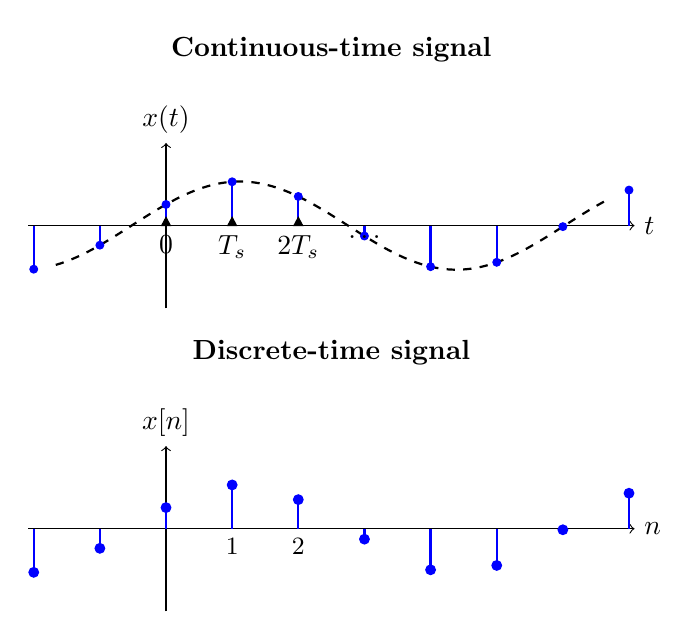
\begin{tikzpicture}[scale=0.7]
        % Define sampling period
        \def\Ts{1.2}
        \def\amplitude{0.8}
        
        % Continuous signal plot
        \begin{scope}[yshift=5.5cm]
            \draw[->] (-2.5,0) -- (8.5,0) node[right] {$t$};
            \draw[->] (0,-1.5) -- (0,1.5) node[above] {$x(t)$};
            \node[above] at (3,2.8) {\textbf{Continuous-time signal}};
            
            % Draw continuous signal (sine wave)
            \draw[thick, dashed, black] plot[smooth, domain=-2:8, samples=200] (\x, {\amplitude*sin(deg(\x*0.8 + 0.5))});
            
            % Sampling points
            \foreach \n in {-2,-1,0,1,2,3,4,5,6,7} {
                \pgfmathsetmacro{\t}{\n * \Ts}
                \pgfmathsetmacro{\y}{\amplitude*sin(deg(\t*0.8 + 0.5))}
                \draw[blue, thick] (\t,0) -- (\t,\y);
                \filldraw[blue] (\t,\y) circle (2pt);
            }
            
            % Sampling period markers on x-axis
            \node[below] at (0,0) {$0$};
            \node[below] at (\Ts,0) {$T_s$};
            \node[below] at (2*\Ts,0) {$2T_s$};
            \node[below] at (3*\Ts,0) {$\ldots$};
            
            % Diamond markers (manually drawn)
            \filldraw[black] (0,0.15) -- (0.08,0) -- (0,0) -- (-0.08,0) -- cycle;
            \filldraw[black] (\Ts,0.15) -- (\Ts+0.08,0) -- (\Ts,0) -- (\Ts-0.08,0) -- cycle;
            \filldraw[black] (2*\Ts,0.15) -- (2*\Ts+0.08,0) -- (2*\Ts,0) -- (2*\Ts-0.08,0) -- cycle;
        \end{scope}
        
        % Discrete signal plot
        \begin{scope}
            \draw[->] (-2.5,0) -- (8.5,0) node[right] {$n$};
            \draw[->] (0,-1.5) -- (0,1.5) node[above] {$x[n]$};
            \node[above] at (3,2.8) {\textbf{Discrete-time signal}};
            
            % Draw discrete samples (at same x-positions as continuous graph)
            \foreach \n in {-2,-1,0,1,2,3,4,5,6,7} {
                \pgfmathsetmacro{\t}{\n * \Ts}
                \pgfmathsetmacro{\y}{\amplitude*sin(deg(\t*0.8 + 0.5))}
                \draw[blue, thick] (\t,0) -- (\t,\y);
                \filldraw[blue] (\t,\y) circle (2.5pt);
            }
            
            % Label x-axis with integer indices (only 1 and 2, at same positions as continuous)
            \node[below] at (\Ts,0) {\small $1$};
            \node[below] at (2*\Ts,0) {\small $2$};
        \end{scope}
    \end{tikzpicture}
    \caption{Sampling process: conversion from continuous-time signal $x(t)$ to discrete-time signal $x[n]$. The top plot shows the continuous signal with sampling instants marked, and the bottom plot shows the resulting discrete sequence.}
    \label{fig:sampling_process}
\end{figure}

\subsection{Signal Reconstruction with Sinc Interpolation}

Once a signal has been sampled according to the Nyquist-Shannon theorem, the original continuous signal can be perfectly reconstructed from its discrete samples. This reconstruction is achieved through \textbf{sinc interpolation}, which uses the sinc function to interpolate between sample points.

The sinc function is defined as:
\begin{equation}
\text{sinc}(t) = \frac{\sin(\pi t)}{\pi t}
\label{eq:sinc}
\end{equation}
with the special case $\text{sinc}(0) = 1$ (by L'Hôpital's rule).

The reconstruction formula, also known as the \textbf{Whittaker-Shannon interpolation formula}, expresses the continuous signal $x(t)$ as a weighted sum of sinc functions centered at each sample point:
\begin{equation}
x(t) = \sum_{n=-\infty}^{\infty} x[n] \cdot \text{sinc}\left(\frac{t - nT_s}{T_s}\right)
\label{eq:reconstruction}
\end{equation}

where:
\begin{itemize}
    \item $x[n]$ are the discrete samples
    \item $T_s$ is the sampling period
    \item Each sinc function is centered at a sampling instant $nT_s$
    \item The sinc function has zeros at all other sampling instants, ensuring that $x(t)$ equals $x[n]$ at $t = nT_s$
\end{itemize}

This reconstruction works because:
\begin{enumerate}
    \item At each sampling instant $t = nT_s$, only the sinc function centered at that point contributes (all others are zero), so $x(nT_s) = x[n]$.
    \item Between sampling points, the sinc functions smoothly interpolate the signal values.
    \item In the frequency domain, the sinc function acts as an ideal low-pass filter, removing all frequency components above the Nyquist frequency while preserving those below it.
\end{enumerate}

\begin{tcolorbox}[colback=blue!5!white, colframe=blue!75!black, title=\textbf{Curious Fact: Band-Limited Signals and Perfect Reconstruction}]
Since sinc interpolation acts as a low-pass filter (removing all frequencies above the Nyquist frequency $f_N = f_s/2$), if we have a band-limited signal with maximum frequency $f_{\text{max}}$ lower than the Nyquist frequency, then no frequencies are going to be removed and therefore, the result is a theoretically perfect reconstruction.
\end{tcolorbox}

\subsection{Aliasing}

\textbf{Aliasing} is a distortion phenomenon that occurs when a signal is sampled at a rate that is too low (below the Nyquist rate). When aliasing occurs, high-frequency components of the signal are "folded back" or "aliased" into lower frequencies, making them indistinguishable from actual low-frequency components in the sampled signal.

\subsubsection{Why Aliasing Occurs}

In the frequency domain, sampling creates periodic replicas of the signal's spectrum at integer multiples of the sampling frequency. When the sampling frequency $f_s$ is less than $2f_{\text{max}}$, these replicas overlap. The overlapping high-frequency components appear as lower frequencies in the sampled signal, causing aliasing.

For example, consider a signal with frequency $f = 8$ Hz sampled at $f_s = 10$ Hz:
\begin{itemize}
    \item The Nyquist frequency is $f_N = f_s/2 = 5$ Hz
    \item The signal frequency (8 Hz) is above the Nyquist frequency
    \item The aliased frequency is $f_{\text{alias}} = f_s - f = 10 - 8 = 2$ Hz
    \item The sampled signal incorrectly appears to have a 2 Hz component instead of the original 8 Hz
\end{itemize}

\subsubsection{Consequences of Aliasing}

Once aliasing occurs, the original signal cannot be perfectly reconstructed because the high-frequency information has been irretrievably mixed with lower frequencies. This is why the Nyquist-Shannon theorem requires sampling at or above the Nyquist rate to ensure perfect reconstruction.

\begin{tcolorbox}[colback=blue!5!white, colframe=blue!75!black, title=\textbf{Curious Fact: The Wagon Wheel Effect}]
A classic example of aliasing in everyday life is the \textbf{wagon wheel effect} (also known as the stroboscopic effect) seen in videos. When a wheel with spokes rotates at a certain speed and is filmed at a fixed frame rate, the wheel can appear to rotate backward, slowly, or even stand still. This occurs because the wheel's rotation frequency is being undersampled by the camera's frame rate. The high-frequency rotation is aliased into a lower apparent frequency, creating the illusion of reverse or slow motion. This is a temporal aliasing effect, where time (rather than space) is being sampled.
\end{tcolorbox}

These are the three different sampling scenarios:

\begin{itemize}
    \item \textbf{Adequate sampling} ($f_s > 2f_{\text{max}}$): The signal can be perfectly reconstructed.
    \item \textbf{Nyquist rate sampling} ($f_s = 2f_{\text{max}}$): The minimum sampling rate that theoretically allows perfect reconstruction.
    \item \textbf{Insufficient sampling} ($f_s < 2f_{\text{max}}$): Aliasing occurs, and the original signal cannot be recovered.
\end{itemize}


\subsection{Exercise: Determining Minimum Sampling Rate}

Consider the following signal:
\begin{equation}
x(t) = \cos(100\pi t) + \sin(200\pi t) + \cos(500\pi t + \pi/4) + 7
\label{eq:exercise_signal}
\end{equation}

\textbf{Problem:} Determine the minimum sampling rate required to perfectly reconstruct this signal.

\textbf{Solution:}

To find the minimum sampling rate, we need to identify the maximum frequency component in the signal. Let's analyze each term:

\begin{itemize}
    \item $\cos(100\pi t)$: 
    \begin{align*}
    \text{Angular frequency: } \omega_1 &= 100\pi \text{ rad/s} \\
    \text{To convert to frequency: } f_1 &= \omega_1 \times \frac{1 \text{ cycle}}{2\pi \text{ rad}} \\
    &= 100\pi \text{ rad/s} \times \frac{1 \text{ cycle}}{2\pi \text{ rad}} \\
    &= \frac{100\cancel{\pi \text{ rad}}/\text{s} \times 1 \text{ cycle}}{2\cancel{\pi \text{ rad}}} \\
    &= \frac{100}{2} \frac{\text{cycle}}{\text{s}} = 50 \text{ cycles/s} = 50 \text{ Hz}
    \end{align*}
    
    \item $\sin(200\pi t)$: $f_2 = \frac{200\pi}{2\pi} = 100$ Hz
    
    \item $\cos(500\pi t + \pi/4)$: $f_3 = \frac{500\pi}{2\pi} = 250$ Hz
    
    \item $7$: This is a constant (DC component) with frequency $f_0 = 0$ Hz
\end{itemize}

The maximum frequency in the signal is $f_{\text{max}} = 250$ Hz (from the $\cos(500\pi t + \pi/4)$ term).

According to the Nyquist-Shannon theorem, the minimum sampling rate (Nyquist rate) is:
\begin{equation}
f_s \geq 2f_{\text{max}} = 2 \times 250 = 500 \text{ Hz}
\end{equation}

Therefore, the minimum sampling rate required is \textbf{500 Hz}.

Figure~\ref{fig:aliasing_exercise} demonstrates the signal reconstruction process using \textbf{sinc interpolation} (Whittaker-Shannon interpolation formula) for three different sampling scenarios. The reconstruction is performed using the formula:
\begin{equation}
x(t) = \sum_{n=-\infty}^{\infty} x[n] \cdot \text{sinc}\left(\frac{t - nT_s}{T_s}\right)
\end{equation}
where $\text{sinc}(t) = \frac{\sin(\pi t)}{\pi t}$ and $T_s = 1/f_s$ is the sampling period.

Each row of the figure shows three plots: (1) the original continuous signal, (2) the sampled signal with sample points marked, and (3) the reconstructed signal using sinc interpolation overlaid with the original for comparison. The three rows correspond to:
\begin{itemize}
    \item \textbf{Adequate sampling} ($f_s = 600$ Hz $> 2f_{\text{max}}$): The reconstructed signal perfectly matches the original, demonstrating perfect reconstruction when sampling above the Nyquist rate.
    \item \textbf{Nyquist rate sampling} ($f_s = 500$ Hz $= 2f_{\text{max}}$): The reconstructed signal matches the original, showing that the Nyquist rate is the theoretical minimum for perfect reconstruction.
    \item \textbf{Insufficient sampling} ($f_s = 300$ Hz $< 2f_{\text{max}}$): The reconstructed signal does not match the original due to aliasing, demonstrating that perfect reconstruction is impossible when sampling below the Nyquist rate.
\end{itemize}

\begin{figure}[H]
    \centering
    \includegraphics[width=0.95\textwidth]{img/aliasing_exercise.png}
    \caption{Signal reconstruction using sinc interpolation for $x(t) = \cos(100\pi t) + \sin(200\pi t) + \cos(500\pi t + \pi/4) + 7$ with $f_{\text{max}} = 250$ Hz. Each row shows: original signal (left), sampled signal (center), and reconstructed signal using sinc interpolation (right). The three rows demonstrate adequate sampling (600 Hz), Nyquist rate (500 Hz), and insufficient sampling (300 Hz) where aliasing prevents perfect reconstruction.}
    \label{fig:aliasing_exercise}
\end{figure}


\section*{Lecture 004}
\section{Entropy: Concept and Estimation}

\subsection{Noise}
\textbf{Noise} is any unwanted signal of random nature that modifies the intensity of the original signal to be perceived.

In the real world, signals are affected by uncontrollable elements that generate noise. This noise is typically superimposed as \textbf{additive noise}:

\begin{equation}
S(t) = f(t) + r(t)
\label{eq:additive_noise}
\end{equation}

where $S(t)$ is the received signal, $f(t)$ is the original signal, and $r(t)$ is the noise component.

The first stage in signal processing focuses on identifying and eliminating noisy artifacts, though complete elimination is usually not feasible. The random nature of noise means that signals with noise are not deterministic but rather \textbf{stochastic processes}, where repeated measurements of the same signal produce different results.

\subsubsection{Types of Noise}

\paragraph{Atmospheric Noise}
Atmospheric noise comes from electrical signals derived from natural discharges that occur under the ionosphere. Storms or electrical charges in clouds are sources of this type of noise, which generally affects communication systems using the radio spectrum more significantly. Approximately, the power of atmospheric noise is inversely proportional to frequency. Thus, atmospheric noise has greater impact on low and medium frequency bands, while lower power noise affects VHF and UHF bands. As a result, atmospheric noise affects AM communication bands and decreases significantly at TV and FM frequencies. Beyond 30 MHz, atmospheric noise has less negative impact than the receiver's own noise.

\paragraph{Man-Made Noise}
This refers to electrical artifacts generated by sources such as automobiles, electric motors, switches, high-voltage lines, etc. It is also known as \textbf{industrial noise}. The intensity of these noisy signals is greater in large urban centers and industrial areas. In these areas, noise of this nature prevails over other noise sources in the frequency range between 1 MHz and 600 MHz.

\paragraph{Impulsive or Shot Noise}
This type of noise causes the appearance of anomalous values (outliers) in the signal. It is characterized by a sudden increase in intensity during a short period of time. Generally, its origin is an external agent to the information system: a lightning strike or interference from a motor spark. However, it should not be confused with atmospheric or man-made noise, as the duration of these is more prolonged in time.

\paragraph{Galactic Noise}
It originates from disturbances produced beyond the Earth's atmosphere. The main sources of galactic noise are the sun and other stars.

\begin{itemize}
    \item \textbf{Solar}: The sun is a major source of energy emission in the form of electromagnetic radiation. These signals affect telecommunications systems. The frequency range of these emissions is very wide, including bands commonly used for radio communication systems. The intensity of the emission produced by the sun varies cyclically, with a period of approximately eleven years. At the highest levels, this radiation can make some frequency bands unusable.
    \item \textbf{Cosmic}: Like the sun, other stars near our planet emit energy in the form of electromagnetic radiation that can affect our signals and communication systems.
\end{itemize}

\paragraph{Thermal Noise}
This noise source is due to the random agitation of electrons in the elements of an electronic circuit. This movement could only be canceled under absolute zero temperature conditions. Therefore, it is an unavoidable noise source that will always be present in a signal acquisition and processing system. The movement of electrons increases as the temperature of the conductor increases, giving rise to small electrical currents. This noisy signal is distributed over a wide range of frequencies, so it will always affect the system to some degree, despite carrying out different filtering stages.

\paragraph{Flicker Noise or 1/f Noise}
It is called 1/f because its power decays below 1 kHz when frequency increases. Therefore, it has greater impact on low frequencies. The physical causes of this type of noise are not entirely clear. It originates in elements such as transistors or resistors, and it is hypothesized that it is due to intermodulation processes in these elements.

\subsubsection{Signal-to-Noise Ratio (SNR)}

When an information source is affected by noisy artifacts, the \textbf{Signal-to-Noise Ratio (SNR)} quantitatively indicates the quality of the signal of interest. This ratio is defined as the quotient between the power of the received signal and the estimated noise power. A value greater than unity (1) indicates a greater presence of the signal compared to the noise. The relationship between these power terms is generally expressed in decibels (dB).

\begin{equation}
\text{SNR} = 10\log_{10}\left(\frac{P_S}{P_N}\right)
\label{eq:snr}
\end{equation}

where:
\begin{itemize}
    \item $P_S$ corresponds to the signal power.
    \item $P_N$ corresponds to the noise power.
\end{itemize}

\paragraph{Example:}

Consider a communication system where the signal power is $P_S = 100$ and the noise power is $P_N = 10$. The SNR is calculated as:

\begin{align*}
\text{SNR} &= 10\log_{10}\left(\frac{P_S}{P_N}\right) \\
          &= 10\log_{10}\left(\frac{100}{10}\right) \\
          &= 10\log_{10}(10) \\
          &= 10 \times 1 = 10 \text{ dB}
\end{align*}

This means the signal power is 10 times greater than the noise power (a ratio of 10:1), resulting in an SNR of 10 dB.

\textbf{Interpretation of SNR values:}
\begin{itemize}
    \item \textbf{SNR greater than 0 dB}: Signal power exceeds noise power (good quality)
    \item \textbf{SNR = 0 dB}: Signal and noise powers are equal
    \item \textbf{SNR lower than 0 dB}: Noise power exceeds signal power (poor quality)
    \item \textbf{SNR = 20 dB}: Signal is 100 times stronger than noise (excellent quality)
    \item \textbf{SNR = 3 dB}: Signal is approximately 2 times stronger than noise (minimum acceptable for many applications)
\end{itemize}

\subsection{Entropy}
Signals contain information and are affected by various noise sources. In this context, the concept of \textbf{entropy} arises. Similar to physics, the term refers to the complexity of the signal. The addition of noise increases the degree of complexity of a signal, resulting in higher entropy.

In information theory, \textbf{entropy} is defined as the amount of information from a random source (on average). Therefore, entropy serves to \textbf{characterize a random variable}. Signals can be modeled as a sequence of realizations of a random variable over time (stochastic process), so we will see how to extend the definition of entropy to random elements of this nature.

\subsubsection{Shannon's Entropy Definition}

Given a discrete random variable $X$ that takes values from the set $\{x_1, x_2, \ldots, x_M\}$ with probability distribution $P(X = x_i) = p_i$, Shannon defined entropy as:

\begin{equation}
H(X) = E\{-\log_2[P(X)]\} = \sum_{i=1}^{M} -\log_2[P(x_i)] \cdot P(x_i) = \sum_{i=1}^{M} -p_i \log_2(p_i)
\label{eq:shannon_entropy}
\end{equation}

where $-\log_2[P(x_i)]$ is interpreted as the \textbf{quantity of information} (or \textbf{self-information}) associated with outcome $x_i$.

\begin{tcolorbox}[colback=blue!5!white, colframe=blue!75!black, title=\textbf{Curious Fact: What Does $E$ Mean?}]
The capital $E$ denotes the \textbf{expected value} (also called expectation or mean). For a discrete random variable, the expected value of a function $g(X)$ is calculated as:
\begin{equation}
E[g(X)] = \sum_{i=1}^{M} g(x_i) \cdot P(x_i)
\end{equation}
In the entropy formula, $E\{-\log_2[P(X)]\}$ means we take the expected value of the information content $-\log_2[P(X)]$, which gives us the average information across all possible outcomes.
\end{tcolorbox}

\subsubsection{Understanding the Formula}

The key insight is that \textbf{less probable values carry more information} (surprise effect) compared to more probable values. For example:
\begin{itemize}
    \item If an event is very likely ($p_i \approx 1$), then $-\log_2(p_i) \approx 0$: we learn little new information.
    \item If an event is very unlikely ($p_i \approx 0$), then $-\log_2(p_i)$ is large: we learn a lot of new information.
\end{itemize}

Entropy $H(X)$ is the \textbf{expected value} (average) of this information content across all possible outcomes.

\subsubsection{Example: Bernoulli Distribution}

Consider a random variable $X$ with only two possible outcomes, $\{x_1, x_2\}$ (a \textbf{Bernoulli distribution}). Let $P(X = x_1) = p$ and $P(X = x_2) = 1-p$. The entropy is:

\begin{equation}
H(X) = -p \log_2(p) - (1-p) \log_2(1-p)
\label{eq:bernoulli_entropy}
\end{equation}

The entropy reaches its \textbf{maximum value of 1} when $p = 0.5$. In this case, both events have equal probability, and on average we obtain the same amount of information from $X$. When $p$ approaches 0 or 1, the entropy approaches 0, meaning we can almost predict the outcome with certainty, so we learn little new information.

\textbf{Concrete Example:} Consider a fair coin flip where $p = 0.5$:
\begin{align*}
H(X) &= -0.5 \log_2(0.5) - 0.5 \log_2(0.5) \\
     &= -0.5 \cdot (-1) - 0.5 \cdot (-1) \\
     &= 0.5 + 0.5 = 1
\end{align*}
This means each coin flip provides an entropy of 1 on average. If the coin is biased (e.g., $p = 0.9$ for heads), then:
\begin{align*}
H(X) &= -0.9 \log_2(0.9) - 0.1 \log_2(0.1) \\
     &\approx 0.469
\end{align*}
The entropy is lower because we can predict the outcome more easily (heads is very likely), so we learn less information.

Figure~\ref{fig:bernoulli_entropy} shows the variation of entropy $H(X)$ as a function of the probability $P(X = x_1) = p$ for a Bernoulli distribution. The curve is symmetric and reaches its maximum value of 1 when $p = 0.5$, demonstrating that uncertainty (entropy) is highest when both outcomes are equally probable.

\begin{figure}[H]
    \centering
    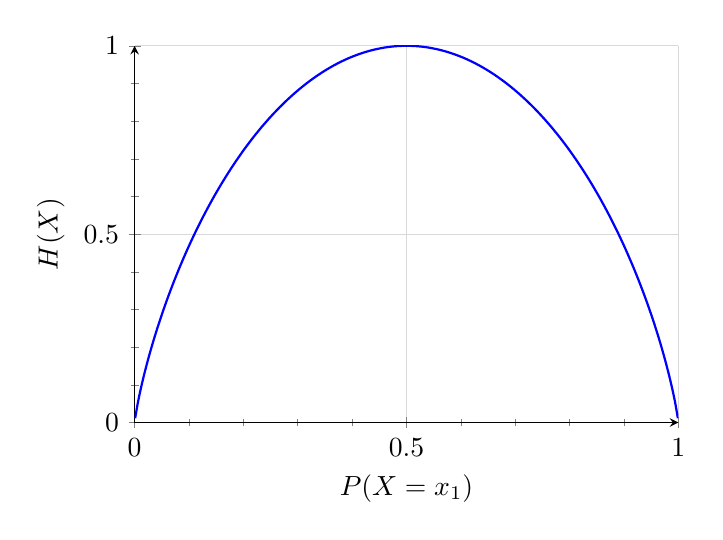
\begin{tikzpicture}
        \begin{axis}[
            width=0.7\textwidth,
            height=0.525\textwidth,
            xlabel={$P(X = x_1)$},
            ylabel={$H(X)$},
            xmin=0, xmax=1,
            ymin=0, ymax=1,
            grid=major,
            grid style={gray!30},
            axis lines=left,
            xtick={0, 0.5, 1},
            ytick={0, 0.5, 1},
            minor xtick={0.1,0.2,0.3,0.4,0.6,0.7,0.8,0.9},
            minor ytick={0.1,0.2,0.3,0.4,0.6,0.7,0.8,0.9},
            minor grid style={gray!10},
            legend pos=north east,
        ]
        \addplot[
            domain=0.001:0.999,
            samples=200,
            smooth,
            thick,
            blue,
        ] {-x*log2(x) - (1-x)*log2(1-x)};
        \end{axis}
    \end{tikzpicture}
    \caption{Entropy $H(X)$ as a function of probability $P(X = x_1) = p$ for a Bernoulli distribution. The entropy reaches its maximum value of 1 when $p = 0.5$ (equal probability for both outcomes) and approaches 0 when $p$ approaches 0 or 1 (certain outcomes).}
    \label{fig:bernoulli_entropy}
\end{figure}

\subsection{Signals as Stochastic Processes}

Signals can be modeled mathematically as a set of random variables (a \textbf{stochastic process}). For example, a voice signal of a certain duration can be viewed as a finite time series, where each sample represents a realization of a random variable.

Including new samples in the series increases the information content, showing that process entropy depends on its length. Therefore, it makes sense to measure the variation of signal entropy due to the inclusion of a new sample. This is called the \textbf{entropy rate} or \textbf{differential entropy}.

\subsubsection{Entropy of a Stochastic Process}

Consider a signal of length $N$ as a sequence of $N$ random variable realizations: $\mathbf{x} = x_1, x_2, \ldots, x_N$. Figure~\ref{fig:signal_sequence} illustrates this concept, showing a signal where each sample $x_i$ represents a realization of a random variable at time index $i$.

\begin{figure}[H]
    \centering
    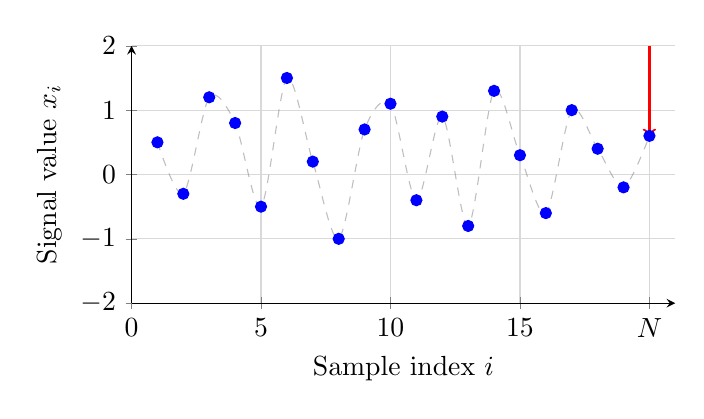
\begin{tikzpicture}
        \begin{axis}[
            width=0.7\textwidth,
            height=0.4\textwidth,
            xlabel={Sample index $i$},
            ylabel={Signal value $x_i$},
            xmin=0, xmax=21,
            ymin=-2, ymax=2,
            grid=major,
            grid style={gray!30},
            axis lines=left,
            xtick={0,5,10,15,20},
            xticklabels={0,5,10,15,$N$},
            ytick={-2,-1,0,1,2},
        ]
        % Generate some random-looking signal values
        \addplot[
            only marks,
            mark=*,
            mark size=2pt,
            blue,
        ] coordinates {
            (1,0.5) (2,-0.3) (3,1.2) (4,0.8) (5,-0.5)
            (6,1.5) (7,0.2) (8,-1.0) (9,0.7) (10,1.1)
            (11,-0.4) (12,0.9) (13,-0.8) (14,1.3) (15,0.3)
            (16,-0.6) (17,1.0) (18,0.4) (19,-0.2) (20,0.6)
        };
        \addplot[
            smooth,
            dashed,
            gray,
            opacity=0.5,
        ] coordinates {
            (1,0.5) (2,-0.3) (3,1.2) (4,0.8) (5,-0.5)
            (6,1.5) (7,0.2) (8,-1.0) (9,0.7) (10,1.1)
            (11,-0.4) (12,0.9) (13,-0.8) (14,1.3) (15,0.3)
            (16,-0.6) (17,1.0) (18,0.4) (19,-0.2) (20,0.6)
        };
        % Add annotation for N
        \node[above] at (axis cs:20,2.2) {$N=20$};
        \draw[->, red, thick] (axis cs:20,2.0) -- (axis cs:20,0.6);
        \end{axis}
    \end{tikzpicture}
    \caption{A signal of length $N=20$ as a sequence of random variable realizations. Each point $(i, x_i)$ represents a sample where $i$ is the time index and $x_i$ is the realization of the random variable at that time.}
    \label{fig:signal_sequence}
\end{figure}

The entropy $H_N$ of this stochastic process is:

\begin{equation}
\begin{split}
H_N &= E\{-\log_2[p(x_1, x_2, \ldots, x_N)]\} \\
&= -\int_{-\infty}^{\infty} \log_2[p(x_1, x_2, \ldots, x_N)] \cdot p(x_1, x_2, \ldots, x_N) \, dx_1 \ldots dx_N
\end{split}
\label{eq:stochastic_entropy}
\end{equation}

where $p(x_1, x_2, \ldots, x_N)$ is the joint probability density function (PDF) of the variables composing the stochastic process.

\begin{tcolorbox}[colback=blue!5!white, colframe=blue!75!black, title=\textbf{Note: Computational Complexity}]
Computing entropy using the stochastic process formula is \textbf{much more computationally expensive} than ApEn:

\begin{itemize}
    \item \textbf{Stochastic process entropy}: Requires estimating an $N$-dimensional joint PDF and computing an $N$-dimensional integral. The complexity grows exponentially with $N$ (curse of dimensionality), making it impractical for long signals.
    \item \textbf{ApEn}: Works with fixed-length subseries ($m$ is typically 2-3), requiring only pattern matching. Complexity is approximately $O(N^2)$, which is manageable even for long signals.
\end{itemize}

This computational advantage is one of the main reasons why ApEn is widely used in practice.
\end{tcolorbox}

\subsubsection{Entropy Rate}

The \textbf{entropy rate} $E_N$ of the signal is defined as:

\begin{equation}
E_N = \lim_{N \to \infty} (H_{N+1} - H_N)
\label{eq:entropy_rate}
\end{equation}

This represents the change in entropy when a new sample is added to an infinitely long sequence.

\begin{tcolorbox}[colback=blue!5!white, colframe=blue!75!black, title=\textbf{Note}]
The entropy rate measures how much entropy increases (on average) when you add one more sample to a long signal.
\end{tcolorbox}

\subsubsection{Approximate Entropy (ApEn)}

There are various methods for estimating signal entropy. \textbf{Approximate Entropy (ApEn)} is one such estimation procedure. The algorithm involves estimating the entropy of subseries of length $m$ and $m+1$. The final entropy value is obtained by taking the difference between these two estimations.

\paragraph{Methodology:}

Consider an original time series $\mathbf{x} = [x_1, x_2, \ldots, x_N]$.

\textbf{Step 1: Extract subseries.} Extract all subseries of length $m$, denoted as $x_i^{(m)} = [x_i, x_{i+1}, \ldots, x_{i+m-1}]$ for $i = 1, 2, \ldots, N-m+1$.

\textbf{Step 2: Find similar subseries.} Given a tolerance $r$, count the number of subseries $N^{(m)}(i)$ that are similar to $x_i^{(m)}$, where similarity is determined by a distance metric $d[x_i^{(m)}, x_j^{(m)}] \leq r$.

\textbf{Step 3: Calculate probability.} The probability of finding a subseries similar to $x_i^{(m)}$ in the original series is:
\begin{equation}
C^{(m)}(i) = \frac{N^{(m)}(i)}{N - m + 1}
\label{eq:apen_probability}
\end{equation}
where $N - m + 1$ is the total number of subseries of length $m$ that can be extracted from the original series.

\textbf{Step 4: Estimate entropy.} The term $C^{(m)}(i)$ provides a discrete estimation of the probability density function. Using Shannon's entropy definition, the entropy of the process represented by $x^{(m)}$ is:
\begin{equation}
H_N^{(m)} = -\frac{1}{N - m + 1} \sum_{i=1}^{N-m+1} \log_2[C^{(m)}(i)]
\label{eq:apen_entropy}
\end{equation}

The Approximate Entropy is then calculated as:
\begin{equation}
\text{ApEn}(m, r, N) = H_N^{(m)} - H_N^{(m+1)}
\label{eq:apen}
\end{equation}

\begin{tcolorbox}[colback=blue!5!white, colframe=blue!75!black, title=\textbf{Note: ApEn vs. Entropy Rate}]
Approximate Entropy (ApEn) is \textbf{not exactly the same} as the entropy rate, but they are related concepts:

\begin{itemize}
    \item \textbf{Entropy rate} $E_N = \lim_{N \to \infty} (H_{N+1} - H_N)$ measures the change in entropy when adding one more \textbf{sample} to the sequence.
    \item \textbf{ApEn} $= H_N^{(m)} - H_N^{(m+1)}$ measures the change in entropy when increasing the \textbf{subseries length} from $m$ to $m+1$.
\end{itemize}

ApEn is an \textbf{approximation} of the entropy rate. Instead of computing the theoretical entropy rate (which requires the full joint PDF), ApEn estimates it by analyzing patterns in subseries of different lengths. Both measure how entropy changes with sequence length, but ApEn uses a practical, pattern-based approach rather than the theoretical limit.
\end{tcolorbox}

\paragraph{Example:}

Consider a time series $\mathbf{x} = [1.0, 1.2, 0.9, 1.1, 1.3, 0.8]$ with $N = 6$. Let $m = 2$ and $r = 0.2$.

\textbf{Step 1: Extract subseries of length $m = 2$:}
\begin{itemize}
    \item $x_1^{(2)} = [1.0, 1.2]$
    \item $x_2^{(2)} = [1.2, 0.9]$
    \item $x_3^{(2)} = [0.9, 1.1]$
    \item $x_4^{(2)} = [1.1, 1.3]$
    \item $x_5^{(2)} = [1.3, 0.8]$
\end{itemize}

\textbf{Step 2: Find similar subseries.} Using the Chebyshev distance (maximum absolute difference between corresponding elements), we count how many subseries are within tolerance $r = 0.2$ of each $x_i^{(2)}$. Two subseries are similar if $d[x_i^{(m)}, x_j^{(m)}] = \max_k |x_{i+k} - x_{j+k}| \leq r$.

For example, comparing $x_1^{(2)} = [1.0, 1.2]$ with $x_4^{(2)} = [1.1, 1.3]$:
\begin{align*}
d[x_1^{(2)}, x_4^{(2)}] &= \max(|1.0 - 1.1|, |1.2 - 1.3|) \\
                         &= \max(0.1, 0.1) = 0.1 \leq 0.2
\end{align*}
Since $0.1 \leq 0.2$, these subseries are similar.

Results for all subseries:
\begin{itemize}
    \item For $x_1^{(2)} = [1.0, 1.2]$: $N^{(2)}(1) = 2$ (matches itself and $x_4^{(2)} = [1.1, 1.3]$)
    \item For $x_2^{(2)} = [1.2, 0.9]$: $N^{(2)}(2) = 1$ (only itself)
    \item For $x_3^{(2)} = [0.9, 1.1]$: $N^{(2)}(3) = 1$ (only itself)
    \item For $x_4^{(2)} = [1.1, 1.3]$: $N^{(2)}(4) = 2$ (matches itself and $x_1^{(2)}$)
    \item For $x_5^{(2)} = [1.3, 0.8]$: $N^{(2)}(5) = 1$ (only itself)
\end{itemize}

\textbf{Step 3: Calculate probabilities.} With $N - m + 1 = 6 - 2 + 1 = 5$ total subseries:
\begin{align*}
C^{(2)}(1) &= \frac{2}{5} = 0.4 \\
C^{(2)}(2) &= \frac{1}{5} = 0.2 \\
C^{(2)}(3) &= \frac{1}{5} = 0.2 \\
C^{(2)}(4) &= \frac{2}{5} = 0.4 \\
C^{(2)}(5) &= \frac{1}{5} = 0.2
\end{align*}

\textbf{Step 4: Estimate entropy.}
\begin{align*}
H_6^{(2)} &= -\frac{1}{5} \sum_{i=1}^{5} \log_2[C^{(2)}(i)] \\
          &= -\frac{1}{5}[\log_2(0.4) + \log_2(0.2) + \log_2(0.2) + \log_2(0.4) + \log_2(0.2)] \\
          &\approx -\frac{1}{5}[-1.32 - 2.32 - 2.32 - 1.32 - 2.32] \\
          &\approx 1.92
\end{align*}

Similarly, we would compute $H_6^{(3)}$ for subseries of length $m+1 = 3$, and then:
$$\text{ApEn}(2, 0.2, 6) = H_6^{(2)} - H_6^{(3)}$$

\begin{tcolorbox}[colback=yellow!5!white, colframe=yellow!75!black, title=\textbf{Takeaway: Why is ApEn Useful?}]
Approximate Entropy is a practical and powerful tool for signal analysis because:

\begin{itemize}
    \item \textbf{Practical estimation}: It provides a computationally feasible way to estimate entropy without requiring knowledge of the full probability distribution, making it applicable to real-world signals.
    \item \textbf{Pattern detection}: By analyzing subseries patterns, ApEn can detect regularity and predictability in signals, which is useful for characterizing signal complexity.
    \item \textbf{Noise robustness}: The tolerance parameter $r$ allows ApEn to be robust to noise, focusing on overall patterns rather than exact matches.
    \item \textbf{Wide applications}: ApEn is widely used in biomedical signal processing (EEG, ECG), time series analysis, and any domain where quantifying signal complexity or regularity is important.
    \item \textbf{Comparative analysis}: It enables comparison of entropy between different signals or different segments of the same signal, helping identify changes in signal characteristics.
\end{itemize}
\end{tcolorbox}

\subsection{Entropy in Images}

The entropy value of a signal can be interpreted as its degree of uncertainty. Equivalently, it reflects the capacity to predict a future state or value from the knowledge or observation of previous signal values. A higher entropy value reflects greater complexity and chaos in the signal under study.

As a result, entropy gives us an idea of the level of noise impact on a signal. If we take a sample of the same signal under the same conditions but at different time instants, the signal with higher entropy will be the one with a higher noise level.

\subsubsection{Images vs. One-Dimensional Signals}

The nature and mathematical modeling of images are different from one-dimensional time-dependent signals. An image does not have an implicit time variable, as occurs in a voice signal or an electrocardiogram, but rather represents light captured at each spatial position. Additionally, image information is represented in two dimensions.

Therefore, in images, just as in time series we characterized the rate of entropy increase with respect to new samples, we could think of an entropy rate with respect to the unit area represented. For entropy estimation in an image, the histogram of intensity levels is used. The final estimation is obtained as the entropy of the random variable characterized by this histogram.

As with one-dimensional signals, entropy will tend to increase, or at least remain the same, if the image area considered for estimation is enlarged. Thus, lower entropy values will be associated with repetitive patterns in the image that lead to a histogram with marked peaks (texture). In contrast, entropy increases if there is greater variability in the intensity values observed in the image, with no marked patterns producing a flatter histogram. In this sense, it follows that noise contributes to increasing the entropy of the image, as it causes the variability of the observed intensity levels to increase.

\subsection{Mathematical Characterization of Noise: Stochastic Processes}

The term \textbf{stochastic process} has been previously used in this topic to refer to a random signal. In our case, any signal will be the result of the combination of the signal of interest and an unwanted signal, of random and chaotic nature, which contributes to increasing entropy. This unwanted signal is noise.

Therefore, the resulting signal is, in itself, a random signal. Just as happens with a random variable, from which we take a sample and obtain values according to a probability density function, the signals we handle are realizations of a stochastic process. Each time we extract a sample from the information source, we obtain a different signal.

In this section, a formal definition of stochastic process is provided that allows understanding the modeling and characterization of noise in signal processing.

\subsubsection{Random Variables}

A random variable is characterized by the following three elements:

\begin{itemize}
    \item \textbf{Sample space}: The set of all possible outcomes that can be observed in the realization of an experiment.
    \item \textbf{Set of events}: Subset of the sample space.
    \item \textbf{Probability law}: Assignment of probability to each of the observable events.
\end{itemize}

\paragraph{Example: Rolling a Fair Die}

Consider the experiment of rolling a fair six-sided die:

\begin{itemize}
    \item \textbf{Sample space}: $\Omega = \{1, 2, 3, 4, 5, 6\}$ (all possible outcomes)
    \item \textbf{Set of events}: Examples include:
    \begin{itemize}
        \item Event $A$: "Rolling an even number" = $\{2, 4, 6\}$
        \item Event $B$: "Rolling a number greater than 4" = $\{5, 6\}$
        \item Event $C$: "Rolling a 3" = $\{3\}$
    \end{itemize}
    \item \textbf{Probability law}: For a fair die, each outcome has equal probability:
    \begin{itemize}
        \item $P(1) = P(2) = P(3) = P(4) = P(5) = P(6) = \frac{1}{6}$
        \item $P(A) = P(\{2, 4, 6\}) = \frac{3}{6} = \frac{1}{2}$
        \item $P(B) = P(\{5, 6\}) = \frac{2}{6} = \frac{1}{3}$
    \end{itemize}
\end{itemize}

\paragraph{Example: Signal Intensity Measurement}

In signal processing, consider measuring the intensity of a signal at a specific time:

\begin{itemize}
    \item \textbf{Sample space}: $\Omega = [0, 255]$ (all possible intensity values, e.g., for an 8-bit image)
    \item \textbf{Set of events}: Examples include:
    \begin{itemize}
        \item Event $D$: "Intensity between 100 and 150" = $[100, 150]$
        \item Event $E$: "Intensity greater than 200" = $(200, 255]$
    \end{itemize}
    \item \textbf{Probability law}: Defined by a probability density function (PDF) $f(x)$ that assigns probabilities to intervals, such as:
    \begin{itemize}
        \item $P(D) = \int_{100}^{150} f(x) \, dx$
        \item $P(E) = \int_{200}^{255} f(x) \, dx$
    \end{itemize}
\end{itemize}

\subsubsection{Stochastic Processes}

A stochastic process can be viewed as a random variable for which the result of an experiment is given in the form of a signal. In the same way as a random variable, it is characterized by the three elements mentioned: sample space, set of events, and probability assignment law.

In practice, as previously mentioned in this topic, we will have noisy signals that, from a mathematical point of view, will be modeled as a stochastic process. The noise component will be assumed to be additive, so the captured signal will have the following form:

\begin{equation}
y(t) = x(t) + \varepsilon(t)
\label{eq:noisy_signal}
\end{equation}

where:
\begin{itemize}
    \item $x(t)$ reflects the signal of interest.
    \item $\varepsilon(t)$ corresponds to the noise.
\end{itemize}

\paragraph{Example: Sinusoidal Signal with Gaussian Noise}

Consider, for example, that the signal of interest corresponds to a tone of frequency $f$ and that the noise component follows a Gaussian distribution with zero mean and variance $\sigma^2$.

In Figure~\ref{fig:stochastic_signal}, we can see this target signal (top) and a realization of the stochastic process that corresponds to the observed signal (bottom).

\begin{figure}[H]
    \centering
    \includegraphics[width=0.7\textwidth]{img/stocastic_001.png}
    \caption{Comparison of a clean sinusoidal signal (top) and a noisy realization of the stochastic process (bottom). The noise component gives the signal a random nature that prevents us from knowing its exact value at any instant $t$.}
    \label{fig:stochastic_signal}
\end{figure}

As can be seen, the noise component gives the signal a random nature that prevents us from knowing its exact value at any instant $t$. In order to characterize the stochastic process, the objective will be to know its statistical properties. Probability distribution and density functions allow us to model the process statistically.

These functions are given as follows:

\begin{itemize}
    \item \textbf{Distribution function}: $F_X(x,t) = P(X(t) \leq x)$
    \item \textbf{Probability density function}: $f_X(x,t) = \frac{dF_X(x,t)}{dx}$
\end{itemize}

From these functions, the stationarity of the process can be defined:

\begin{itemize}
    \item A process is stationary in \textbf{strict sense} if the probability density function that characterizes the process does not vary with time. That is, for a constant $c$ such that $c > 0$, the following will hold: $f_X(x,t) = f_X(x,t+c)$
    \item A process is stationary in \textbf{wide sense} if the statistical moments that characterize it (mean, variance, etc.) do not vary with respect to time.
\end{itemize}

\paragraph{Example: Strict-Sense Stationarity}

Consider a process $X(t) = A \sin(2\pi f t + \phi)$, where $A$ and $\phi$ are random variables, and $f$ is a constant frequency. If $A$ and $\phi$ are independent, with $A$ having a fixed distribution and $\phi$ uniformly distributed on $[0, 2\pi]$, then the PDF of $X(t)$ at any time $t$ is the same (it depends only on the distribution of $A$ and $\phi$, not on $t$). This process is stationary in strict sense because $f_X(x,t) = f_X(x,t+c)$ for any $c$.

\paragraph{Example: Wide-Sense Stationarity}

Consider white noise $\varepsilon(t)$ with zero mean and constant variance $\sigma^2$:
\begin{itemize}
    \item Mean: $E[\varepsilon(t)] = 0$ (constant, independent of $t$)
    \item Variance: $\text{Var}[\varepsilon(t)] = \sigma^2$ (constant, independent of $t$)
    \item Autocorrelation: $E[\varepsilon(t)\varepsilon(t+\tau)] = \sigma^2 \delta(\tau)$ (depends only on $\tau$, not on $t$)
\end{itemize}
This process is stationary in wide sense because its statistical moments (mean and variance) do not vary with time, even though we may not know the full PDF.

\paragraph{Example: Non-Stationary Process}

Consider a process $Y(t) = t + \varepsilon(t)$, where $\varepsilon(t)$ is white noise. The mean of this process is $E[Y(t)] = t$, which clearly varies with time. Therefore, this process is \textbf{not stationary} (neither in strict sense nor in wide sense) because its statistical properties change over time.

\paragraph{Example: Non-Stationary Signal with Trend}

Let us return to the previous example. In this case, the captured signal shows, in addition to Gaussian noise, another component that causes a clear trend over time. Figure~\ref{fig:nonstationary_trend} shows this new example.

\begin{figure}[H]
    \centering
    \includegraphics[width=0.7\textwidth]{img/stochastic_002.png}
    \caption{Non-stationary signal with a trend component. The signal exhibits both Gaussian noise and a clear trend over time, making its statistical properties vary along the temporal axis.}
    \label{fig:nonstationary_trend}
\end{figure}

As a result of this trend, the statistical properties of the signal do not remain constant along the temporal axis, so it cannot be considered a stationary signal. It will be necessary to eliminate the noise component that causes this trend to remove the non-stationarity present in our information.


\section*{Lecture 005}
\section{Anomaly Detection and Cancellation}

\subsection{Definition of Anomaly}

\textbf{Anomaly detection} aims to identify atypical values in the information source, commonly known as \textbf{outliers}. These are defined as unusual patterns that do not conform to expected behavior. The appearance of outliers in a signal or image reflects the existence of noise, typically impulsive noise caused by, for example: a peak value in a nearby electric field, or instabilities in the capture procedure, such as sudden camera movement.

Anomaly detection has direct applications in various practical scenarios:

\begin{itemize}
    \item \textbf{Intrusion detection in networks}. Identification of atypical patterns in network traffic that may indicate an attack.
    
    \item \textbf{Medical diagnosis}. Recognition of lesions with low incidence in the population that may indicate the existence of some pathology.
    
    \item \textbf{Fraudulent transaction detection}. The vast majority of transactions are legitimate, and only a small proportion correspond to fraudulent activities.
    
    \item \textbf{Customer churn prediction in large companies}. In banking, insurance, and telecommunications sectors, a small portion of customers abandon the company, so the identification of these behaviors can be performed using anomaly detection techniques.
\end{itemize}

\subsection{Types of Anomalies}

\subsubsection{Point Anomalies}

When an individual sample can be considered notably different from the rest of the data, it can be taken as an outlier. This type of anomaly is the simplest and the focus of most research work on this topic.

A clear example corresponding to a real scenario would be credit card fraud. If we look at a variable such as the transaction amount, those transactions for which the amount is very high compared to the average of previous transactions are susceptible to being point anomalies and, therefore, suspicious of fraud. Thus, a point anomaly is expressed by the appearance of peak values that deviate excessively from the set of values we observe.

Figure~\ref{fig:point_anomaly} shows a signal in which one of the samples takes a value that is not observed in any other sample. This is clearly a candidate sample for being an anomaly.

\begin{figure}[H]
    \centering
    \includegraphics[width=0.8\textwidth]{img/anomaly_001.png}
    \caption{Example of a point anomaly in a signal: a sharp spike (highlighted in black) that deviates significantly from the normal signal pattern.}
    \label{fig:point_anomaly}
\end{figure}

\subsubsection{Contextual Anomalies}

If a data sample is anomalous in a specific context (but not otherwise), it is called a \textbf{contextual anomaly}. The notion of context is given by the nature of the data. Each data sample is defined considering the following attributes:

\begin{itemize}
    \item \textbf{Contextual attributes}: These are used to determine the context (or neighborhood) for that sample. They are given by the nature of the data source. For example, in temperature monitoring systems, the time of day or season are contextual attributes. In network traffic analysis, the timestamp or day of the week serve as contextual attributes. In image processing, the spatial coordinates $(x, y)$ of a pixel are contextual attributes.
    
    \item \textbf{Behavioral attributes}: These define the non-contextual character of an instance. That is, they represent the value of the sample. In the temperature monitoring example, the actual temperature reading is a behavioral attribute. In network traffic analysis, the number of packets or bytes transmitted is a behavioral attribute. In image processing, the pixel intensity or color values are behavioral attributes.
\end{itemize}

Anomalous behavior is determined using the values of behavioral attributes within a specific context. A data instance could be a contextual anomaly in a given context, but an identical data instance (in terms of behavioral attributes, i.e., its value) could be considered normal in a different context. This property is key to identifying contextual and behavioral attributes for a contextual anomaly detection technique.

Unlike point anomalies, where only a comparison of available data samples is performed to identify an atypical value, in temporal signals (time series) and images, context is taken into account to define an abnormal value. For example, in an image, it is possible to identify an anomalous pixel if its intensity is very different from that of neighboring pixels. Similarly, in a time series, the neighborhood of a point provides the contextual information necessary to identify an anomalous value, as exemplified in Figure~\ref{fig:contextual_anomaly}. In this figure, we can see that the series takes similar values to the anomaly at some point, but the context indicates that in this case it is an atypical sample.

\begin{figure}[H]
    \centering
    \includegraphics[width=0.8\textwidth]{img/anomaly_002.png}
    \caption{Example of a contextual anomaly in a time series: a spike (highlighted in black) that appears anomalous given its context, even though similar values occur elsewhere in the signal.}
    \label{fig:contextual_anomaly}
\end{figure}

\subsubsection{Collective Anomalies}

If a collection of related data instances is anomalous with respect to the entire dataset, it is called a \textbf{collective anomaly}. The individual data instances in a collective anomaly may not be anomalies by themselves, but their joint occurrence as a collection is anomalous.

Figure~\ref{fig:collective_anomaly} illustrates an example of a collective anomaly in an electrocardiographic signal. The highlighted region denotes an anomaly because the signal takes approximately the same value for an unusually long time. However, that value itself is not an anomaly.

\begin{figure}[H]
    \centering
    \includegraphics[width=0.8\textwidth]{img/anomaly_003.png}
    \caption{Example of a collective anomaly in an ECG signal: a highlighted region (in red) where the signal maintains approximately the same value for an unusually long duration, forming an anomalous pattern.}
    \label{fig:collective_anomaly}
\end{figure}

\subsection{Anomaly Detection Methods}

Unlike conventional classification problems, where a labeled training set and a test set are available, anomaly detection has multiple possible configurations depending on the labels available in the dataset. We can distinguish between three main types:

\subsubsection{Supervised Methods}

Training data contains labeled samples (both normal and anomalous). A classifier is trained to learn patterns that distinguish anomalies from normal data, then classifies new unlabeled data. This approach requires known and correctly labeled anomalies, which limits its applicability. Common algorithms include Support Vector Machines (SVM) and Artificial Neural Networks (ANN). Typically used in applications like fraud detection or medical diagnosis where anomalies are well-defined.

\begin{figure}[H]
    \centering
    \includegraphics[width=0.8\textwidth]{img/supervised.png}
    \caption{Supervised anomaly detection workflow}
    \label{fig:supervised}
\end{figure}

\subsubsection{Semi-Supervised Methods}

Training data contains only normal (non-anomalous) samples. The model learns the normal pattern, then identifies anomalies as deviations from this learned pattern. This approach is known as \textbf{one-class classifiers}. Common algorithms include one-class SVM, autoencoders, Gaussian mixture models, and kernel-based density estimation. More practical than supervised methods since it only requires normal samples, not labeled anomalies.

\begin{figure}[H]
    \centering
    \includegraphics[width=0.8\textwidth]{img/semi-supervised.png}
    \caption{Semi-supervised anomaly detection workflow}
    \label{fig:semi_supervised}
\end{figure}

\subsubsection{Unsupervised Methods}

No labeled data is required. The algorithm scores data based solely on intrinsic properties (distances or densities) to identify what is normal versus atypical. This is the most flexible approach. The output is typically a continuous score reflecting the degree of abnormality, allowing instances to be ranked by their anomaly score. Semi-supervised methods also produce continuous scores for ranking suspicious cases.

\begin{figure}[H]
    \centering
    \includegraphics[width=0.8\textwidth]{img/non-supervised.png}
    \caption{Unsupervised anomaly detection workflow}
    \label{fig:unsupervised}
\end{figure}

\subsection{Anomaly Removal}

The following explains the most common unsupervised procedures for removing anomalies in signals.

\subsubsection{Median Filter}

The median filter has been commonly employed on 1D and 2D signals for removing impulsive noise. These artifacts are easily recognized through visual inspection of the signal, as they are associated with peak values that stand out notably from the rest of the signal (point anomaly) or from the immediate neighborhood (contextual anomaly, since the atypical value would be inconsistent with those in its environment).

In images, this type of anomaly is known as \textbf{salt \& pepper noise}, as the effect it generates is that of randomly placed pixels that take extreme intensity values (1 or 0).

The median filter is an operation applied point by point using a sliding window. The size of this window is determined by the user. For one-dimensional signals such as time series, it is a window of length $N$, while in images the window is defined in both coordinates and is of size $N \times N$. The value of $N$ is odd, since the window is centered on the point of the signal to be filtered. Thus, the resulting value at this point is given by the median of the points considered by the window.

As can be seen from its definition, the filter does not create new signal values, but selects one of the incoming values as output. The median filter is very similar to an average filter that would obtain, for each window, the mean value of the pixels or points considered. This operation is equivalent to using a low-pass filter in frequency, so rapid variations of the signal, reflected as significant contrasts in an image, are smoothed by the filter.

\subsubsection{Statistical Techniques}

A common technique for detecting and correcting anomalies relies on using the \textbf{probability density function} of the data. Given the density function $f(x)$, where $x$ is one of the values the corresponding random variable can take, a measure quantifying the degree of anomaly for a sample $x_1$ can be obtained as the inverse of $f(x_1)$.

Values that are very improbable will tend to be identified as atypical (outliers). Therefore, an appropriate strategy must be used for their treatment, such as eliminating them or estimating their value as the mean of neighboring points.

\begin{tcolorbox}[colback=blue!5!white, colframe=blue!75!black, title=\textbf{Curious Fact: What is a Probability Density Function?}]
The \textbf{probability density function} (PDF) $f(x)$ describes how the probability is distributed over the possible values of a continuous random variable. For a given value $x$, the function $f(x)$ tells us the relative likelihood that the random variable will take that value. 

Key properties:
\begin{itemize}
    \item The PDF is always non-negative: $f(x) \geq 0$ for all $x$
    \item The area under the entire curve equals 1: $\int_{-\infty}^{\infty} f(x) \, dx = 1$
    \item Higher values of $f(x)$ indicate that $x$ is more likely to occur
    \item Lower values of $f(x)$ indicate that $x$ is less likely (more unusual/anomalous)
\end{itemize}

In anomaly detection, values with very low probability density (low $f(x)$) are considered outliers, as they represent rare or unusual occurrences in the data.
\end{tcolorbox}

\textbf{Example:} Consider a signal with values following a normal distribution with mean $\mu = 0$ and standard deviation $\sigma = 1$. For this specific distribution, the probability density function is:
\begin{equation}
f(x) = \frac{1}{\sqrt{2\pi}} e^{-\frac{x^2}{2}}
\end{equation}
Note that this is the PDF formula for a \textbf{standard normal distribution}. Different probability distributions have different PDF formulas. The general form for a normal distribution with mean $\mu$ and standard deviation $\sigma$ is:
\begin{equation}
f(x) = \frac{1}{\sigma\sqrt{2\pi}} e^{-\frac{(x-\mu)^2}{2\sigma^2}}
\end{equation}

Figure~\ref{fig:pdf_anomaly} illustrates the probability density function for the standard normal distribution, showing how the PDF value decreases as we move away from the mean, making outliers easier to identify.

\begin{figure}[H]
    \centering
    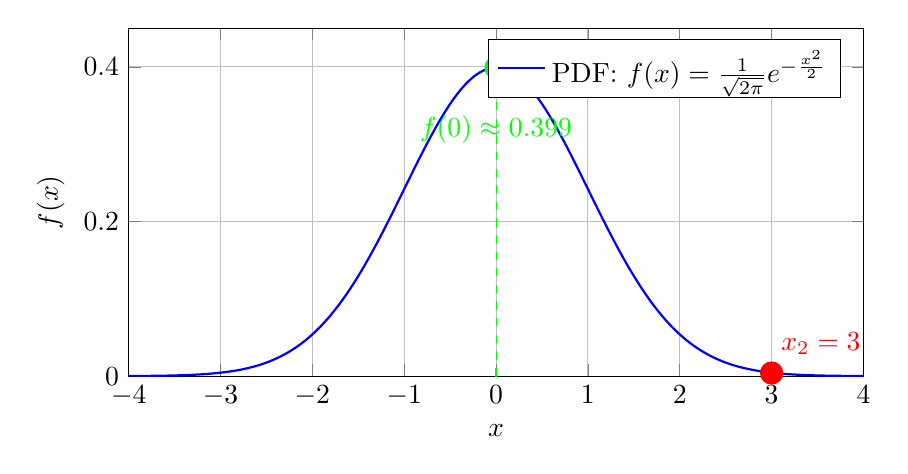
\begin{tikzpicture}
        \begin{axis}[
            width=0.9\textwidth,
            height=6cm,
            xlabel={$x$},
            ylabel={$f(x)$},
            xmin=-4, xmax=4,
            ymin=0, ymax=0.45,
            grid=major,
            legend pos=north east,
            samples=200
        ]
            % Plot the normal distribution PDF
            \addplot[thick, blue, domain=-4:4] {1/sqrt(2*pi) * exp(-x^2/2)};
            \addlegendentry{PDF: $f(x) = \frac{1}{\sqrt{2\pi}} e^{-\frac{x^2}{2}}$}
            
            % Mark x1 = 0 (normal sample)
            \addplot[mark=*, mark size=4pt, color=green, only marks] coordinates {(0, 0.399)};
            \node[above, color=green] at (axis cs: 0, 0.45) {$x_1 = 0$};
            \node[below, color=green] at (axis cs: 0, 0.35) {$f(0) \approx 0.399$};
            \draw[dashed, green] (axis cs: 0, 0) -- (axis cs: 0, 0.399);
            
            % Mark x2 = 3 (outlier)
            \addplot[mark=*, mark size=4pt, color=red, only marks] coordinates {(3, 0.004)};
            \node[above right, color=red] at (axis cs: 3, 0.015) {$x_2 = 3$};
            \node[below, color=red] at (axis cs: 3, -0.02) {$f(3) \approx 0.004$};
            \draw[dashed, red] (axis cs: 3, 0) -- (axis cs: 3, 0.004);
            
            % Add vertical lines to x-axis
            \draw[green, thick] (axis cs: 0, -0.01) -- (axis cs: 0, 0.01);
            \draw[red, thick] (axis cs: 3, -0.01) -- (axis cs: 3, 0.01);
        \end{axis}
    \end{tikzpicture}
    \caption{Probability density function of a standard normal distribution ($\mu = 0$, $\sigma = 1$). The green point at $x_1 = 0$ shows a normal sample with high probability density ($f(0) \approx 0.399$), while the red point at $x_2 = 3$ shows an outlier with very low probability density ($f(3) \approx 0.004$).}
    \label{fig:pdf_anomaly}
\end{figure}

\textbf{Step 1:} Evaluate the probability density for a normal sample $x_1 = 0$ (at the mean):
\begin{equation}
f(0) = \frac{1}{\sqrt{2\pi}} e^{0} \approx 0.399
\end{equation}

\textbf{Step 2:} Calculate the anomaly degree for $x_1$:
\begin{equation}
\text{Anomaly degree} = \frac{1}{f(0)} \approx \frac{1}{0.399} \approx 2.5 \quad \text{(low anomaly)}
\end{equation}

The anomaly degree of 2.5 is considered "low" because it corresponds to a value at the mean of the distribution (most likely value). In practice, anomaly degrees are evaluated \textbf{relative to other samples} in the dataset or compared to a threshold. Common thresholds are based on:
\begin{itemize}
    \item \textbf{Standard deviations}: Values beyond 2-3 standard deviations from the mean
    \item \textbf{Percentiles}: Values below the 1st percentile or above the 99th percentile
    \item \textbf{Relative comparison}: Comparing anomaly degrees across all samples and identifying those significantly higher than the median
\end{itemize}

\textbf{Step 3:} Evaluate the probability density for a potential outlier $x_2 = 3$ (three standard deviations away):
\begin{equation}
f(3) = \frac{1}{\sqrt{2\pi}} e^{-\frac{9}{2}} \approx 0.004
\end{equation}

\textbf{Step 4:} Calculate the anomaly degree for $x_2$:
\begin{equation}
\text{Anomaly degree} = \frac{1}{f(3)} \approx \frac{1}{0.004} \approx 250 \quad \text{(high anomaly)}
\end{equation}

\textbf{Step 5:} Since $x_2$ has a very high anomaly degree (250 vs 2.5), it is identified as an outlier. The comparison shows that $x_2$ has an anomaly degree \textbf{100 times higher} than $x_1$ ($250/2.5 = 100$), indicating it is extremely unlikely and anomalous. In practice, a threshold would be established (e.g., anomaly degree $> 50$ or $> 100$) to automatically flag outliers. Treatment options include: (1) eliminating the value, or (2) replacing it with the mean of its neighboring points.

\subsubsection{Threshold-Based Outlier Detection}

An alternative statistical strategy identifies outliers as values located at the extremes of the domain of a function $f(x)$. This approach defines two threshold values $x_a$ and $x_b$ such that:
\begin{equation}
P(x \leq x_a) = P(x \geq x_b) = P_{\text{min}}
\label{eq:threshold}
\end{equation}
where $P_{\text{min}}$ is a predefined minimum probability threshold. A sample $x_1$ is considered an anomaly if $x_1 < x_a$ or $x_1 > x_b$.

\textbf{Global Application (Point Anomalies):} When applied globally, the function $f(x)$ represents the entire set of available samples (e.g., all points in a time series or all pixels in an image). This approach detects \textbf{point anomalies}, where an individual sample is notably different from the overall dataset.

\textbf{Local Application (Contextual Anomalies):} To identify \textbf{contextual anomalies}, the method is applied within a local environment or neighborhood of the point being studied. Here, $f(x)$ is defined solely based on the neighborhood of the point being evaluated. This involves using a \textbf{sliding window} centered on the target point, similar to how a median filter operates, to define the local context and establish local thresholds $x_a$ and $x_b$ for that specific neighborhood.

\subsubsection{Practical Considerations}

Additionally, both methods based on $f(x)$ require initially setting a \textbf{decision threshold}: 
\begin{itemize}
    \item For the inverse density method: to compare the obtained anomaly score against a threshold
    \item For the threshold-based method: to define the $P_{\text{min}}$ value that identifies the extreme values of a distribution
\end{itemize}

\begin{tcolorbox}[colback=blue!5!white, colframe=blue!75!black, title=\textbf{Important: User-Defined Threshold}]
This threshold determines the definition of anomaly in our dataset and must be established by the user. The choice of threshold directly affects which samples are classified as anomalies, making it a critical parameter in the detection process.
\end{tcolorbox}

In the definition of methods based on the use of the probability density function $f(x)$, knowledge of this function has been assumed. However, in practice, this function is typically \textbf{unknown}, so it is necessary to apply \textbf{estimation techniques} to obtain an approximation of it. The following are some techniques that can be used for estimating this function.

\subsubsection{Estimation Techniques}

\paragraph{Histogram}

This represents the simplest technique. From the samples of a variable, it is discretized by dividing its domain into a limited number of intervals of equal size, identified by their midpoint. These points represent the discrete values that the variable can take. Thus, the frequency (probability) associated with each possible value is obtained from the total initial dataset by counting the number of samples of the variable that fall into each interval.

The choice of the number of intervals used for discretizing the variable has a very significant influence on the obtained approximation. A number that is too small will result in an excessively simple approximation that does not capture the particularities of the target distribution. However, an excessive number of intervals leads to the resulting estimation presenting discontinuities (null values) and abrupt changes in its profile.

\textbf{Example:} Consider a dataset with 20 samples: $\{1.2, 1.5, 1.8, 2.1, 2.3, 2.4, 2.6, 2.7, 2.9, 3.0, 3.1, 3.2, 3.4, 3.5, 3.7, 3.9, 4.2, 4.5, 4.8, 5.1\}$.

\textbf{Step 1:} Divide the domain into intervals. For example, using 5 intervals of width 1.0:
\begin{itemize}
    \item Interval 1: $[1.0, 2.0)$ with midpoint $1.5$
    \item Interval 2: $[2.0, 3.0)$ with midpoint $2.5$
    \item Interval 3: $[3.0, 4.0)$ with midpoint $3.5$
    \item Interval 4: $[4.0, 5.0)$ with midpoint $4.5$
    \item Interval 5: $[5.0, 6.0)$ with midpoint $5.5$
\end{itemize}

\textbf{Step 2:} Count samples in each interval:
\begin{itemize}
    \item Interval 1: 3 samples $\{1.2, 1.5, 1.8\}$ → frequency $= 3/20 = 0.15$
    \item Interval 2: 7 samples $\{2.1, 2.3, 2.4, 2.6, 2.7, 2.9, 3.0\}$ → frequency $= 7/20 = 0.35$
    \item Interval 3: 6 samples $\{3.1, 3.2, 3.4, 3.5, 3.7, 3.9\}$ → frequency $= 6/20 = 0.30$
    \item Interval 4: 3 samples $\{4.2, 4.5, 4.8\}$ → frequency $= 3/20 = 0.15$
    \item Interval 5: 1 sample $\{5.1\}$ → frequency $= 1/20 = 0.05$
\end{itemize}

\textbf{Step 3:} The estimated probability density function assigns to each midpoint the frequency of its interval. For example, $f(2.5) \approx 0.35$ and $f(5.5) \approx 0.05$. A new sample $x = 5.3$ would fall in interval 5, which has low frequency (0.05), indicating it is likely an anomaly.

Figure~\ref{fig:histogram_estimation} visualizes the histogram estimation, showing the frequency bars for each interval. The low frequency in interval 5 (highlighted in red) indicates that values in this range are anomalous.

\begin{figure}[H]
    \centering
    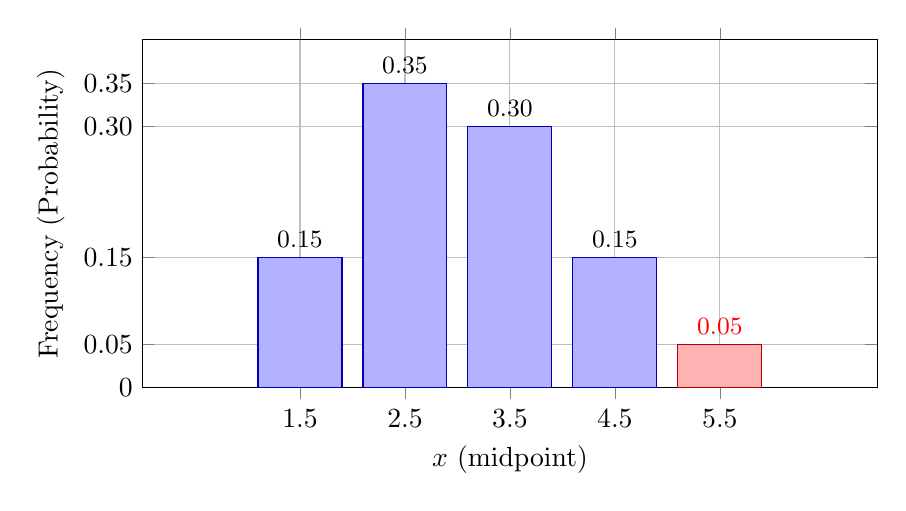
\begin{tikzpicture}
        \begin{axis}[
            width=0.9\textwidth,
            height=6cm,
            xlabel={$x$ (midpoint)},
            ylabel={Frequency (Probability)},
            xmin=1, xmax=6,
            ymin=0, ymax=0.4,
            xtick={1.5, 2.5, 3.5, 4.5, 5.5},
            xticklabels={1.5, 2.5, 3.5, 4.5, 5.5},
            ytick={0, 0.05, 0.15, 0.30, 0.35},
            yticklabels={0, 0.05, 0.15, 0.30, 0.35},
            grid=major,
            bar width=0.8,
            ybar,
            bar shift=0pt,
            enlarge x limits=0.2
        ]
            % Histogram bars
            \addplot[fill=blue!30, draw=blue!70!black] coordinates {
                (1.5, 0.15)
                (2.5, 0.35)
                (3.5, 0.30)
                (4.5, 0.15)
            };
            
            % Anomalous interval (low frequency)
            \addplot[fill=red!30, draw=red!70!black] coordinates {
                (5.5, 0.05)
            };
            
            % Add labels on bars
            \node[above] at (axis cs: 1.5, 0.15) {\small 0.15};
            \node[above] at (axis cs: 2.5, 0.35) {\small 0.35};
            \node[above] at (axis cs: 3.5, 0.30) {\small 0.30};
            \node[above] at (axis cs: 4.5, 0.15) {\small 0.15};
            \node[above, color=red] at (axis cs: 5.5, 0.05) {\small 0.05};
            
            % Mark anomaly region
            \node[below, color=red] at (axis cs: 5.5, -0.02) {\small Anomaly};
        \end{axis}
    \end{tikzpicture}
    \caption{Histogram estimation of probability density function. Each bar represents the frequency (probability) of samples in that interval. The red bar (interval 5) has very low frequency (0.05), indicating anomalous values.}
    \label{fig:histogram_estimation}
\end{figure}

\textbf{Note:} If we had used only 2 intervals, we would lose detail about the distribution shape. If we used 20 intervals (one per sample), many intervals would have zero frequency, creating discontinuities.

\paragraph{Kernel Density Estimation}

Kernel Density Estimation (KDE) is a non-parametric method that provides a smooth estimate of the probability density function. Instead of using fixed intervals like histograms, KDE places a "kernel" (a smooth function, typically a Gaussian) centered at each data point and sums these kernels to create a continuous density estimate.

The estimated density function is given by:
\begin{equation}
\hat{f}(x) = \frac{1}{nh} \sum_{i=1}^{n} K\left(\frac{x - x_i}{h}\right)
\label{eq:kde}
\end{equation}
where $n$ is the number of samples, $h$ is the bandwidth (smoothing parameter), $x_i$ are the data points, and $K$ is the kernel function. A common choice is the Gaussian kernel: $K(u) = \frac{1}{\sqrt{2\pi}} e^{-\frac{u^2}{2}}$.

\begin{tcolorbox}[colback=blue!5!white, colframe=blue!75!black, title=\textbf{Curious Fact: What is a Kernel?}]
A \textbf{kernel} is a smooth, symmetric function that assigns weights to nearby data points. Think of it as a "bump" or "hill" centered at each data point that spreads influence to nearby regions.

Key properties of kernels:
\begin{itemize}
    \item \textbf{Symmetric}: $K(-u) = K(u)$ for all $u$
    \item \textbf{Non-negative}: $K(u) \geq 0$ for all $u$
    \item \textbf{Integrates to 1}: $\int_{-\infty}^{\infty} K(u) \, du = 1$ (ensures the density estimate is valid)
    \item \textbf{Peak at center}: Maximum value occurs at $u = 0$
\end{itemize}

The Gaussian kernel is most common because it's smooth and has infinite support, meaning it gives non-zero weight to all points (though very small for distant points). Other kernel types include uniform, triangular, and Epanechnikov kernels. The kernel essentially "smears" each data point's influence across its neighborhood, creating a smooth density estimate when all kernels are summed together.
\end{tcolorbox}

The bandwidth $h$ plays a crucial role: a small $h$ creates a detailed but noisy estimate, while a large $h$ produces a smoother but potentially oversimplified estimate.

\textbf{Example:} Using the same dataset as before: $\{1.2, 1.5, 1.8, 2.1, 2.3, 2.4, 2.6, 2.7, 2.9, 3.0, 3.1, 3.2, 3.4, 3.5, 3.7, 3.9, 4.2, 4.5, 4.8, 5.1\}$.

\textbf{Step 1:} Choose a bandwidth. For this example, let $h = 0.5$ (moderate smoothing).

\textbf{Step 2:} For any point $x$, calculate the density estimate by summing Gaussian kernels centered at each data point. For example, at $x = 2.5$:
\begin{equation}
\hat{f}(2.5) = \frac{1}{20 \times 0.5} \sum_{i=1}^{20} \frac{1}{\sqrt{2\pi}} e^{-\frac{(2.5 - x_i)^2}{2 \times 0.5^2}}
\end{equation}
This gives a smooth, continuous estimate of the density.

\textbf{Step 3:} For an anomalous point $x = 5.3$, the density estimate will be very low because it is far from most data points. The kernels centered at nearby points (like $x_i = 5.1$) contribute little, and kernels from distant points contribute almost nothing, resulting in $\hat{f}(5.3) \approx 0.02$, indicating an anomaly.

Figure~\ref{fig:kde_estimation} compares the histogram and KDE estimates, showing how KDE provides a smooth continuous curve without discontinuities.

\begin{figure}[H]
    \centering
    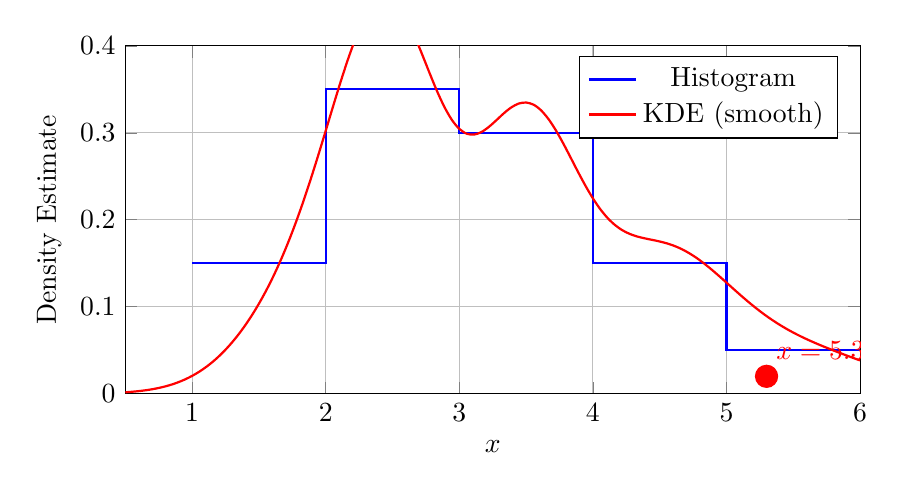
\begin{tikzpicture}
        \begin{axis}[
            width=0.9\textwidth,
            height=6cm,
            xlabel={$x$},
            ylabel={Density Estimate},
            xmin=0.5, xmax=6,
            ymin=0, ymax=0.4,
            grid=major,
            legend pos=north east
        ]
            % Histogram (step function approximation)
            \addplot[thick, blue, const plot, samples=5] coordinates {
                (1, 0.15) (2, 0.15)
                (2, 0.35) (3, 0.35)
                (3, 0.30) (4, 0.30)
                (4, 0.15) (5, 0.15)
                (5, 0.05) (6, 0.05)
            };
            \addlegendentry{Histogram}
            
            % KDE smooth curve (approximation)
            \addplot[thick, red, smooth, samples=100, domain=0.5:6] {
                0.15*exp(-((x-2)^2)/0.5) + 
                0.35*exp(-((x-2.5)^2)/0.3) + 
                0.30*exp(-((x-3.5)^2)/0.3) + 
                0.15*exp(-((x-4.5)^2)/0.5) + 
                0.05*exp(-((x-5.5)^2)/0.8)
            };
            \addlegendentry{KDE (smooth)}
            
            % Mark anomaly region
            \addplot[mark=*, mark size=4pt, color=red, only marks] coordinates {(5.3, 0.02)};
            \node[above right, color=red] at (axis cs: 5.3, 0.02) {$x=5.3$ (anomaly)};
        \end{axis}
    \end{tikzpicture}
    \caption{Comparison of histogram and kernel density estimation. The histogram (blue) shows discrete intervals, while KDE (red) provides a smooth continuous estimate. The point $x=5.3$ has very low density in both methods, indicating an anomaly.}
    \label{fig:kde_estimation}
\end{figure}

\paragraph{Parametric Estimation}

It is assumed that the probability density function that statistically characterizes the variable is of normal type. Therefore, the mean and variance of this distribution are the parameters to be obtained. For this, the estimations derived from the available sample are used:

\begin{tcolorbox}[colback=blue!5!white, colframe=blue!75!black, title=\textbf{Curious Fact: What is "Normal Type"?}]
A \textbf{normal distribution} (also called Gaussian distribution) is a bell-shaped, symmetric probability distribution that is one of the most important distributions in statistics. It is called "normal" because many natural phenomena approximately follow this distribution.

Key characteristics:
\begin{itemize}
    \item \textbf{Bell-shaped curve}: Symmetric around the mean, with a single peak
    \item \textbf{Completely determined by two parameters}: Mean $\mu$ (center) and variance $\sigma^2$ (spread)
    \item \textbf{68-95-99.7 rule}: Approximately 68\% of data falls within 1 standard deviation, 95\% within 2, and 99.7\% within 3 standard deviations of the mean
    \item \textbf{Common in nature}: Many measurements (heights, test scores, measurement errors) tend to follow normal distributions due to the Central Limit Theorem
\end{itemize}

When we say a variable is "of normal type," we mean its probability density function follows the normal distribution formula. This assumption simplifies estimation because we only need to estimate two parameters ($\mu$ and $\sigma^2$) instead of the entire function shape.
\end{tcolorbox}

\begin{equation}
\mu_x = \frac{1}{n} \sum_{i=1}^{n} x_i
\label{eq:mean_est}
\end{equation}

\begin{equation}
\sigma_x^2 = \frac{1}{n} \sum_{i=1}^{n} (x_i - \mu_x)^2
\label{eq:variance_est}
\end{equation}

\textbf{Breaking down the equations:}

\textbf{Equation~\ref{eq:mean_est} (Sample Mean):}
\begin{itemize}
    \item $\mu_x$: The estimated mean (average) of the data
    \item $n$: Total number of samples in the dataset
    \item $\sum_{i=1}^{n}$: Summation symbol, meaning "add up all values from $i=1$ to $i=n$"
    \item $x_i$: The $i$-th individual observation/value in the dataset
    \item $\frac{1}{n}$: Dividing by $n$ to get the average (mean)
\end{itemize}
\textit{In simple terms:} Add up all the values and divide by the number of values to get the average.

\textbf{Equation~\ref{eq:variance_est} (Sample Variance):}
\begin{itemize}
    \item $\sigma_x^2$: The estimated variance (measure of spread/dispersion)
    \item $n$: Total number of samples
    \item $(x_i - \mu_x)$: The difference between each value and the mean (how far each point is from the center)
    \item $(x_i - \mu_x)^2$: Squaring the difference (ensures all values are positive and emphasizes larger deviations)
    \item $\sum_{i=1}^{n}$: Sum all the squared differences
    \item $\frac{1}{n}$: Average of the squared differences
\end{itemize}
\textit{In simple terms:} Calculate how far each value is from the mean, square those distances, then average them. This measures how spread out the data is around the mean.

Once these parameters are estimated, the normal probability density function can be fully specified as:

\begin{equation}
f(x) = \frac{1}{\sigma_x\sqrt{2\pi}} e^{-\frac{(x-\mu_x)^2}{2\sigma_x^2}}
\end{equation}

This parametric approach is simpler than non-parametric methods but requires the assumption that the data follows a normal distribution, which may not always be valid.

Obviously, the main limitation of this method comes from the initial assumption about the shape of the distribution. The error in the estimation will be more significant, therefore, the more the real distribution of the variable differs from the normal profile initially assumed. If the data is highly skewed, multimodal, or has heavy tails, the normal assumption will lead to poor density estimates and consequently, inaccurate anomaly detection.

\paragraph{Kernel Functions (Parzen Method)}

This is a hybrid procedure between histogram-based estimation and parametric estimation. In this case, the estimation of the probability density function is given by the superposition of kernel functions centered at each of the initially observed samples $x_i$. The expression for the estimated function is obtained as follows:

\begin{equation}
\hat{f}(x) = \frac{1}{n} \sum_{i=1}^{n} g(x - x_i, \theta)
\label{eq:parzen}
\end{equation}

where:
\begin{itemize}
    \item $g(x, \theta)$ is the kernel function
    \item $\theta$ represents the set of parameters for this function (e.g., bandwidth $h$ in the Gaussian kernel case)
\end{itemize}

This formulation is equivalent to the Kernel Density Estimation (KDE) method described earlier, where the kernel function $g(x - x_i, \theta)$ corresponds to $K((x-x_i)/h)$ scaled appropriately. The Parzen window method provides a unified framework that bridges discrete histogram methods and continuous parametric approaches.

\textbf{Example:} Using the same dataset: $\{1.2, 1.5, 1.8, 2.1, 2.3, 2.4, 2.6, 2.7, 2.9, 3.0, 3.1, 3.2, 3.4, 3.5, 3.7, 3.9, 4.2, 4.5, 4.8, 5.1\}$ with $n = 20$ samples.

\textbf{Step 1:} Choose a kernel function and its parameters. For this example, we use a Gaussian kernel with bandwidth $h = 0.5$:
\begin{equation}
g(x - x_i, \theta) = g(x - x_i, h) = \frac{1}{h\sqrt{2\pi}} e^{-\frac{(x - x_i)^2}{2h^2}}
\end{equation}

\textbf{Step 2:} To estimate the density at any point $x$, sum the kernel functions centered at each data point. For example, at $x = 2.5$:
\begin{equation}
\hat{f}(2.5) = \frac{1}{20} \sum_{i=1}^{20} \frac{1}{0.5\sqrt{2\pi}} e^{-\frac{(2.5 - x_i)^2}{2 \times 0.5^2}}
\end{equation}
Each term in the sum represents the contribution of one data point $x_i$ to the density estimate at $x = 2.5$. Points closer to 2.5 contribute more (higher kernel value), while distant points contribute less.

\textbf{Step 3:} For an anomalous point $x = 5.3$, most kernel functions centered at the data points will have very small values because $5.3$ is far from most samples. The only significant contribution comes from the kernel centered at $x_i = 5.1$, resulting in $\hat{f}(5.3) \approx 0.02$, indicating an anomaly.

\textbf{Visualization:} The Parzen window method creates a smooth density estimate by placing a "bump" (kernel) at each data point and summing all bumps. The height of the resulting curve at any point $x$ represents the estimated probability density, with low values indicating potential anomalies.

Figure~\ref{fig:parzen_visualization} illustrates the Parzen window method, showing individual kernel functions (Gaussian bumps) centered at sample data points and the resulting density estimate obtained by summing all kernels.

\begin{figure}[H]
    \centering
    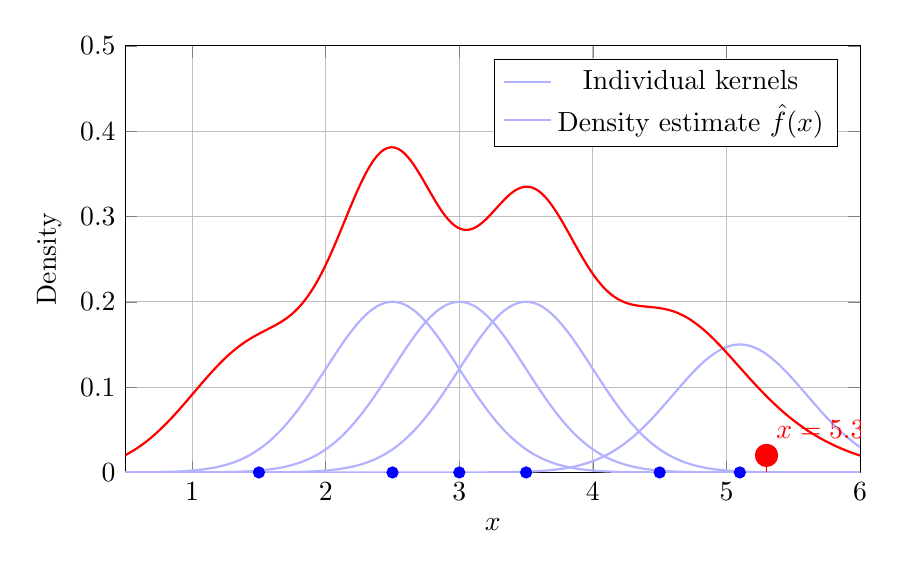
\begin{tikzpicture}
        \begin{axis}[
            width=0.9\textwidth,
            height=7cm,
            xlabel={$x$},
            ylabel={Density},
            xmin=0.5, xmax=6,
            ymin=0, ymax=0.5,
            grid=major,
            legend pos=north east
        ]
            % Sample data points (some representative ones)
            \def\samples{1.5, 2.5, 3.0, 3.5, 4.5, 5.1}
            
            % Draw individual kernels (bumps) at some data points
            \addplot[thick, blue!30, smooth, samples=100, domain=0.5:6] {
                0.2*exp(-((x-2.5)^2)/0.5)
            };
            \addlegendentry{Individual kernels}
            
            \addplot[thick, blue!30, smooth, samples=100, domain=0.5:6] {
                0.2*exp(-((x-3.0)^2)/0.5)
            };
            
            \addplot[thick, blue!30, smooth, samples=100, domain=0.5:6] {
                0.2*exp(-((x-3.5)^2)/0.5)
            };
            
            \addplot[thick, blue!30, smooth, samples=100, domain=0.5:6] {
                0.15*exp(-((x-5.1)^2)/0.5)
            };
            
            % Resulting density estimate (sum of all kernels - approximation)
            \addplot[thick, red, smooth, samples=200, domain=0.5:6] {
                0.15*exp(-((x-1.5)^2)/0.5) + 
                0.35*exp(-((x-2.5)^2)/0.3) + 
                0.30*exp(-((x-3.5)^2)/0.3) + 
                0.15*exp(-((x-4.5)^2)/0.5) + 
                0.05*exp(-((x-5.1)^2)/0.8)
            };
            \addlegendentry{Density estimate $\hat{f}(x)$}
            
            % Mark data points
            \addplot[mark=*, mark size=2pt, color=blue, only marks] coordinates {
                (1.5, 0) (2.5, 0) (3.0, 0) (3.5, 0) (4.5, 0) (5.1, 0)
            };
            
            % Mark anomaly point
            \addplot[mark=*, mark size=4pt, color=red, only marks] coordinates {(5.3, 0.02)};
            \node[above right, color=red] at (axis cs: 5.3, 0.02) {$x=5.3$ (anomaly)};
            
            % Draw vertical line at anomaly
            \draw[dashed, red] (axis cs: 5.3, 0) -- (axis cs: 5.3, 0.02);
        \end{axis}
    \end{tikzpicture}
    \caption{Parzen window method visualization. Individual Gaussian kernels (blue, semi-transparent) are centered at each data point. The resulting density estimate (red curve) is obtained by summing all kernels. The point $x=5.3$ has very low density, indicating an anomaly.}
    \label{fig:parzen_visualization}
\end{figure}

Commonly, a Gaussian normal is used as the kernel function, so that the parameter set $\theta$ is given solely by the variance of the normal, since each kernel function is centered at the corresponding sample. It is common to use the same variance value for all kernel functions, so the estimated probability density function would be obtained as:

\begin{equation}
\hat{f}(x) = \frac{1}{n} \sum_{i=1}^{n} \frac{1}{\sqrt{2\pi\sigma^2}} \exp\left[-\frac{(x-x_i)^2}{2\sigma^2}\right]
\label{eq:gaussian_parzen}
\end{equation}

where $\sigma^2$ is the variance parameter (bandwidth) that controls the width of each Gaussian kernel. As observed, the effect of the variance of the normal kernel functions is similar to the interval size for histogram calculation. In fact, the histogram can be seen as a particular case of kernel-based estimation, in which these functions would be given by uniform pulses of unit height centered at the midpoint of each interval.

\begin{tcolorbox}[colback=blue!5!white, colframe=blue!75!black, title=\textbf{Understanding the Relationship: Histogram vs. Kernel Estimation}]
\textbf{Similarity:} Both histogram interval size and kernel variance control the \textbf{smoothing} of the density estimate:
\begin{itemize}
    \item \textbf{Large histogram intervals} or \textbf{large kernel variance} $\sigma^2$: Produce smoother, less detailed estimates (may oversimplify)
    \item \textbf{Small histogram intervals} or \textbf{small kernel variance} $\sigma^2$: Produce more detailed, potentially noisy estimates (may overfit)
\end{itemize}

\textbf{Histogram as a special case:} A histogram can be viewed as kernel estimation using:
\begin{itemize}
    \item \textbf{Uniform kernels} (rectangular pulses) instead of smooth Gaussian kernels
    \item Kernels of \textbf{unit height} and \textbf{width equal to the interval size}
    \item Kernels \textbf{centered at interval midpoints} rather than at individual data points
\end{itemize}

The key difference is that histograms use \textbf{discrete, non-overlapping} uniform kernels, while kernel density estimation uses \textbf{continuous, overlapping} smooth kernels (typically Gaussian), resulting in a smoother density estimate.
\end{tcolorbox}

A common rule for obtaining an adequate value of the variance of kernel functions is to set it to the following value:

\begin{equation}
\sigma = 1.06 \sigma_x n^{-1/5}
\label{eq:silverman_rule}
\end{equation}

where $\sigma_x$ is the standard deviation of the sample data and $n$ is the number of samples. This is known as \textbf{Silverman's rule of thumb} for bandwidth selection. The factor $1.06$ is optimal for Gaussian kernels when the underlying distribution is approximately normal, and the term $n^{-1/5}$ ensures that the bandwidth decreases as the sample size increases, allowing for more detailed estimates with more data.

This rule provides a good starting point for kernel variance selection, balancing between oversmoothing (too large $\sigma$) and undersmoothing (too small $\sigma$).



\section*{Lecture 006}
\section{Image Processing: Elementary Operations}

There are different operations for image enhancement. In this topic, the focus is on elementary point-to-point operations. These operations are characterized by the fact that the value of a pixel in the processed image is a function solely of the value of that same pixel in the original image. Mathematically, this is expressed as follows:

\begin{equation}
B(x,y) = T(A(x,y))
\label{eq:point_to_point}
\end{equation}

where:
\begin{itemize}
    \item $A(x,y)$ represents the original image, where $A$ is a function that takes spatial coordinates $(x,y)$ as input and returns the pixel intensity value at that location
    \item $B(x,y)$ represents the processed image, where $B$ is the resulting function after applying the transformation
    \item $T$ is the transformation function that maps each pixel value from the original image to a new value in the processed image
    \item The key characteristic is that $B(x,y)$ depends \textbf{only} on $A(x,y)$ at the same coordinates $(x,y)$, not on neighboring pixels
\end{itemize}

\begin{tcolorbox}[colback=blue!5!white, colframe=blue!75!black, title=\textbf{Note: Point-to-Point Operations}]
Point-to-point operations are also known as \textbf{pixel-wise operations} or \textbf{point operations}. They are computationally efficient because each pixel can be processed independently, without requiring information from neighboring pixels. This makes them suitable for parallel processing and real-time applications.
\end{tcolorbox}

To synthesize the information provided in this topic, the following scheme reflects the main concepts:

\begin{itemize}
    \item \textbf{Intensity Adjustment}
    \item \textbf{Histogram Processing}
    \item \textbf{Arithmetic Operators}
\end{itemize}

\subsection{Intensity Adjustment}

Intensity adjustment operations consist of different expressions of the operator $T$ from Equation~\ref{eq:point_to_point}. 

In the context of digital images, $L$ represents the total number of possible intensity levels that a pixel can take. For example:
\begin{itemize}
    \item In an 8-bit grayscale image, $L = 256$ (pixels can take values from 0 to 255)
    \item In a 16-bit grayscale image, $L = 65536$ (pixels can take values from 0 to 65535)
    \item The actual pixel values range from 0 to $L-1$, where 0 represents the darkest level (black) and $L-1$ represents the brightest level (white)
\end{itemize}

Figure~\ref{fig:intensity_adjust} shows some of the most common transformation operations for an image with $L$ different intensity levels. The graph plots output gray levels ($s$) against input gray levels ($r$), ranging from 0 to $L-1$, and displays various transformation curves including Identity, Negative, Logarithmic, Inverse Logarithmic, $n$-th root, and $n$-th power transformations.

\begin{figure}[H]
    \centering
    \includegraphics[width=0.7\textwidth]{img/intensity-adjust.png}
    \caption{Common gray-level transformation functions for point-to-point intensity adjustment operations. The graph shows how different functions map input pixel intensities ($r$) to output pixel intensities ($s$).}
    \label{fig:intensity_adjust}
\end{figure}

\subsubsection{Image Negative}

\textbf{Image negative} (\textit{negativo de una imagen}) represents the inverted image with respect to the original. The mathematical expression of the transformation is given by the following equation:

\begin{equation}
T(u) = L - u
\label{eq:image_negative}
\end{equation}

where $L$ is the maximum intensity level that a pixel can take (e.g., $L = 256$ for 8-bit images, where the maximum value is $L-1 = 255$).

This transformation inverts the gray levels, mapping dark pixels to bright and bright pixels to dark. In the transformation graph, the negative operation appears as a straight diagonal line extending from the top-left corner $(0, L-1)$ to the bottom-right corner $(L-1, 0)$.

\textbf{Example:} In an 8-bit image where $L = 256$, a pixel with intensity $u = 10$ (very dark) becomes $T(10) = 256 - 10 = 246$ (very bright), while a pixel with intensity $u = 246$ becomes $T(246) = 256 - 246 = 10$.

\subsubsection{Logarithmic Transformations}

\textbf{Logarithmic transformations} (\textit{transformaciones logarítmicas}) use a logarithmic function to map pixel intensities. The mathematical expression for logarithmic operators is:

\begin{equation}
T(u) = C \log(1 + u)
\label{eq:logarithmic}
\end{equation}

where $C$ is a constant.

The profile of this operator can be observed in Figure~\ref{fig:intensity_adjust}. As can be seen, this transformation maps a small range of lower intensity values in the input image to a wide range of output values. However, the opposite occurs for higher intensity values, which tend to be concentrated in a narrow range of output values.

Therefore, this transformation is used when we want to expand the range of intensity of dark pixels while simultaneously compressing the brighter pixels together.

The practical utility of this operator can be appreciated in situations where the input image possesses a very wide dynamic range, and its representation would therefore only allow us to distinguish black and white pixels. By applying a logarithmic transformation, the dark regions are expanded, making details in low-intensity areas more visible, while the bright regions are compressed, preventing saturation.

\textbf{Example:} In medical imaging or astronomical images, where the intensity range can span several orders of magnitude, logarithmic transformations help visualize details in both dark and bright regions that would otherwise be lost in a linear representation.

\subsubsection{Power Law Transformations}

\textbf{Power law transformations} (\textit{ley de potencia}), also known as gamma correction, use a power function to map pixel intensities. The transformation function according to the power law is given by the following expression:

\begin{equation}
T(u) = C u^{\gamma}
\label{eq:power_law}
\end{equation}

where $C$ and $\gamma$ are positive constants.

The profile of the functions obtained according to this expression is shown in Figure~\ref{fig:power_law}. As in the case of logarithmic transformations, values of $\gamma$ less than unity tend to expand the range of intensity of darker pixels, while compressing it for brighter pixels.

The advantage of these functions with respect to the logarithmic transformation is the possibility of generating a wide family of transformations simply by varying the parameter $\gamma$. By adjusting $\gamma$, we can achieve different effects:
\begin{itemize}
    \item $\gamma < 1$: Expands dark regions and compresses bright regions (similar to logarithmic transformation)
    \item $\gamma = 1$: Linear transformation (no change, identity function)
    \item $\gamma > 1$: Compresses dark regions and expands bright regions (opposite effect to logarithmic)
\end{itemize}

This flexibility makes power law transformations particularly useful for display calibration, contrast enhancement, and adapting images to different viewing conditions.

\begin{figure}[H]
    \centering
    \includegraphics[width=0.7\textwidth]{img/power.png}
    \caption{Power law transformation curves for different values of $\gamma$. Curves with $\gamma < 1$ expand dark pixel intensities, while curves with $\gamma > 1$ expand bright pixel intensities. The diagonal line represents $\gamma = 1$ (identity transformation).}
    \label{fig:power_law}
\end{figure}

\subsubsection{Piecewise Functions}

The previous functions have a single mathematical expression for the entire domain of application, that is, for any input intensity value. However, it can be interesting to apply different transformations depending on the intensity range of the pixels being operated on. In this situation, \textbf{piecewise operators} (\textit{operadores definidos a trozos o tramos}) are employed.

The main advantage of these functions is that their form or expression can be arbitrarily complex. For example, the input intensity range can be divided into as many segments as desired, defining a specific transformation for each of them.

However, the most relevant disadvantage is that they require a high degree of user involvement for their definition. Generally, a human defines the function through visual inspection of the effect produced by each of the transformations applied to the different segments.

One of the most common applications of this type of function is \textbf{contrast enhancement} in an image. In some situations, the image may have a small dynamic range due to poor scene illumination, the sensor employed, or the lens configuration used in capture. 

Figure~\ref{fig:piecewise} illustrates a piecewise linear transformation function $T(r)$ that selectively enhances contrast in the mid-range of gray levels. The function consists of three segments: a shallow slope for dark regions, a steep slope for intermediate intensities (enhancing contrast), and a moderate slope for bright regions.

\begin{figure}[H]
    \centering
    \includegraphics[width=0.7\textwidth]{img/parts.png}
    \caption{Example of a piecewise linear transformation function $T(r)$ for contrast enhancement. The function selectively expands contrast in the intermediate intensity range (between $r_1$ and $r_2$) while compressing or maintaining contrast in dark and bright regions.}
    \label{fig:piecewise}
\end{figure}

\subsection{Histogram Processing}

As indicated previously, piecewise transformation functions for contrast enhancement require manual definition through trial and error, which can be tedious. An alternative is histogram-based processing, which automatically determines the transformation.

The histogram of an image provides an estimation of the \textbf{probability density function} (\textbf{PDF}) of pixel intensity values. For an image with $L$ intensity levels, the histogram counts how many pixels have each intensity level. The normalized histogram divides these counts by the total number of pixels, giving the probability of each intensity level.

\textbf{Histogram equalization} (\textit{igualación del histograma}) automatically enhances image contrast without user intervention. It redistributes pixel intensities to create a more uniform histogram.

Figure~\ref{fig:histogram_equalization} shows an example of histogram equalization. The transformed histogram becomes more uniform, spreading intensity values across the full range. In contrast, the original histogram concentrates values in a narrow range, resulting in lower contrast.

\begin{figure}[H]
    \centering
    \includegraphics[width=0.95\textwidth]{img/eqist.png}
    \caption{Example of histogram equalization applied to a grayscale image. The top row shows the original image (left) and the equalized image (right). The bottom row shows their corresponding histograms. The equalized histogram exhibits a more uniform distribution with greater dispersion across the full intensity range, resulting in enhanced contrast and improved visibility of details.}
    \label{fig:histogram_equalization}
\end{figure}

\subsection{Arithmetic Operators}

Of the four possible arithmetic operations (addition, subtraction, multiplication, and division), subtraction and addition are the two most useful operators in preprocessing stages for achieving image enhancement.

\subsubsection{Image Enhancement Using the Subtraction Operator}

\textbf{Image enhancement using the subtraction operator} (\textit{realce de imagen mediante el operador resta}) allows highlighting differences between two images. The difference $C(x,y)$ between two images $A(x,y)$ and $B(x,y)$ is obtained by subtracting each pair of pixels in both:

\begin{equation}
C(x,y) = B(x,y) - A(x,y)
\label{eq:image_subtraction}
\end{equation}

This operation enables the detection of differences between images that may appear visually similar. Figure~\ref{fig:arithmetic_subtraction} shows an example where subtraction reveals subtle differences:

\begin{itemize}
    \item \textbf{Top-left:} The original image, where each pixel is encoded using 8 bits, allowing for 256 different intensity levels.
    \item \textbf{Top-right:} An image obtained by setting the fourth bit of each pixel to 0. Visually, there appears to be no difference between this image and the original.
    \item \textbf{Bottom-left:} The result of subtracting the two images (pixel by pixel). This image reveals certain differences between the original and the modified image, despite their apparent similarity.
    \item \textbf{Bottom-right:} The differences from the bottom-left image are further enhanced using histogram equalization, making them more visible.
\end{itemize}

\begin{figure}[H]
    \centering
    \includegraphics[width=0.95\textwidth]{img/arithmetic1.png}
    \caption{Example of image enhancement using subtraction. The top row shows the original image (left) and a modified version with the fourth bit set to 0 (right). The bottom row shows the subtraction result (left) and its histogram-equalized version (right), revealing subtle differences that are not visible in the original comparison.}
    \label{fig:arithmetic_subtraction}
\end{figure}

\subsubsection{Image Smoothing Using the Addition Operator}

\textbf{Image smoothing using the addition operator} (\textit{suavizado de imagen mediante el operador suma}) works similarly to subtraction. The addition operator applied to two or more images consists of adding the intensity values of corresponding pixels in each of them. The interest of this operator lies in its use for obtaining the average image from a set, which allows reducing capture noise.

For a set of $M$ images $A_i(x,y)$ ($i = 1, \ldots, M$), their average is obtained as follows:

\begin{equation}
C(x,y) = \frac{1}{M} \sum_{i=1}^{M} A_i(x,y)
\label{eq:image_averaging}
\end{equation}

Each snapshot $A_i(x,y)$ can be seen as the realization of a \textbf{spatial stochastic process}, a random variable whose observations are images. Therefore, these snapshots are expressed mathematically as:

\begin{equation}
A_i(x,y) = F(x,y) + \eta(x,y)
\label{eq:image_model}
\end{equation}

where:
\begin{itemize}
    \item $F(x,y)$ represents the ideal noise-free image
    \item $\eta(x,y)$ is a stochastic process assumed to be stationary and Gaussian, with zero mean and variance $\sigma^2$
\end{itemize}

If the additive noise $\eta(x,y)$ is assumed uncorrelated between any two snapshots of our set, it can be demonstrated that the average of all of them tends to the image $F(x,y)$:

\begin{equation}
\lim_{M \to \infty} C(x,y) = F(x,y)
\label{eq:averaging_limit}
\end{equation}

The power of the capture noise is attenuated according to a factor $M$ in the resulting average image:

\begin{equation}
\sigma^2_C = \frac{\sigma^2}{M}
\label{eq:noise_reduction}
\end{equation}

where $\sigma^2_C$ is the variance of the noise in the averaged image and $\sigma^2$ is the variance of the noise in a single image.

\begin{tcolorbox}[colback=blue!5!white, colframe=blue!75!black, title=\textbf{Note: Image Alignment Requirement}]
This enhancement strategy based on the attenuation of capture noise assumes that the initial snapshots are perfectly aligned. Otherwise, the final result would show a clear blurring of the edges of the structures in the image.
\end{tcolorbox}

\begin{tcolorbox}[colback=yellow!5!white, colframe=yellow!75!black, title=\textbf{Exercises}]
\textbf{Topics:}
\begin{itemize}
    \item Linear intensity transformations
    \item Power-law transformations
    \item Piecewise linear transformations
    \item Parameter calculation for contrast enhancement
\end{itemize}
\end{tcolorbox}

\textbf{Exercise 1:} Consider an 8-bit image with minimum intensity value $r_{\text{min}} = 35$ and maximum intensity value $r_{\text{max}} = 190$. We want to apply a global linear intensity transformation defined by the equation $s = ar + b$ to obtain a transformed image with minimum intensity value $s_{\text{min}} = 10$ and maximum intensity value $s_{\text{max}} = 240$.

Find the parameters $a$ and $b$ of the linear transformation that maps the original minimum and maximum intensity values exactly to the desired minimum and maximum values.

\textbf{Solution:}

We need to find $a$ and $b$ such that:
\begin{align}
s_{\text{min}} &= ar_{\text{min}} + b \label{eq:ex1_min} \\
s_{\text{max}} &= ar_{\text{max}} + b \label{eq:ex1_max}
\end{align}

Substituting the given values:
\begin{align}
10 &= 35a + b \label{eq:ex1_eq1} \\
240 &= 190a + b \label{eq:ex1_eq2}
\end{align}

To solve for $a$, we subtract equation~\eqref{eq:ex1_eq1} from equation~\eqref{eq:ex1_eq2}:
\begin{align}
240 - 10 &= 190a + b - (35a + b) \\
230 &= 155a \\
a &= \frac{230}{155} = \frac{46}{31} \approx 1.484
\end{align}

Now, substituting $a$ into equation~\eqref{eq:ex1_eq1} to find $b$:
\begin{align}
10 &= 35 \cdot \frac{230}{155} + b \\
10 &= \frac{8050}{155} + b \\
10 &= \frac{1610}{31} + b \\
b &= 10 - \frac{1610}{31} = \frac{310 - 1610}{31} = -\frac{1300}{31} \approx -41.935
\end{align}

\textbf{Verification:}
\begin{itemize}
    \item For $r = 35$: $s = \frac{46}{31} \times 35 - \frac{1300}{31} = \frac{1610 - 1300}{31} = \frac{310}{31} = $ \colorbox{yellow!30}{10}
    \item For $r = 190$: $s = \frac{46}{31} \times 190 - \frac{1300}{31} = \frac{8740 - 1300}{31} = \frac{7440}{31} = $ \colorbox{yellow!30}{240}
\end{itemize}

Therefore, the linear transformation is:
\begin{equation}
s = \frac{46}{31}r - \frac{1300}{31} \approx 1.484r - 41.935
\end{equation}

\textbf{Exercise 2:} Consider an 8-bit grayscale image with intensities $r \in [0, 255]$. A power transformation of the form
\begin{equation}
s = cr^{\gamma}
\end{equation}
is applied, where $c$ and $\gamma$ are positive real constants. It is known that a pixel with original intensity $r = 64$ transforms exactly to $s = 16$.

\begin{enumerate}
    \item Write the equation that relates $c$ and $\gamma$ from the condition $s(64) = 16$.
    \item Suppose that it is desired that the transformation does not modify the maximum intensity value, i.e., that $s(255) = 255$. Use this additional condition to obtain a system of equations and solve for $c$ and $\gamma$, finding a pair of unique numerical values.
\end{enumerate}

\textbf{Solution:}

\textbf{Part 1:} From the condition $s(64) = 16$, we substitute into the transformation equation:
\begin{equation}
16 = c \cdot 64^{\gamma}
\label{eq:ex2_eq1}
\end{equation}
This equation relates $c$ and $\gamma$ but does not uniquely determine either parameter.

\textbf{Part 2:} With the additional condition $s(255) = 255$, we obtain a second equation:
\begin{equation}
255 = c \cdot 255^{\gamma}
\label{eq:ex2_eq2}
\end{equation}

We now have a system of two equations with two unknowns. To solve for $\gamma$, we can eliminate $c$ by dividing equation~\eqref{eq:ex2_eq2} by equation~\eqref{eq:ex2_eq1}:
\begin{align}
\frac{255}{16} &= \frac{c \cdot 255^{\gamma}}{c \cdot 64^{\gamma}} \\
\frac{255}{16} &= \left(\frac{255}{64}\right)^{\gamma} \\
\frac{255}{16} &= \left(\frac{255}{64}\right)^{\gamma}
\end{align}

Taking the natural logarithm of both sides:
\begin{align}
\ln\left(\frac{255}{16}\right) &= \gamma \ln\left(\frac{255}{64}\right) \\
\gamma &= \frac{\ln\left(\frac{255}{16}\right)}{\ln\left(\frac{255}{64}\right)} \\
\gamma &= \frac{\ln(15.9375)}{\ln(3.984375)} \\
\gamma &\approx \frac{2.768}{1.382} \approx 2.002
\end{align}

Now, substituting $\gamma \approx 2.002$ into equation~\eqref{eq:ex2_eq1} to find $c$:
\begin{align}
c &= \frac{16}{64^{\gamma}} \\
c &= \frac{16}{64^{2.002}} \\
c &\approx \frac{16}{4096.5} \approx 0.0039
\end{align}

\textbf{Verification:}
\begin{itemize}
    \item For $r = 64$: $s = 0.0039 \times 64^{2.002} \approx 0.0039 \times 4096.5 \approx $ \colorbox{yellow!30}{16}
    \item For $r = 255$: $s = 0.0039 \times 255^{2.002} \approx 0.0039 \times 65025 \approx $ \colorbox{yellow!30}{254.6} $\approx 255$
\end{itemize}

Therefore, the power-law transformation is approximately:
\begin{equation}
s \approx 0.0039 \cdot r^{2.002}
\end{equation}

\textbf{Exercise 3:} Consider an 8-bit image with intensity levels $r \in [0, 255]$, and a piecewise linear intensity transformation $s = T(r)$ that passes through the points: $(0, 0)$, $(r_1, s_1)$, $(r_2, s_2)$, $(255, 255)$, where $0 < r_1 < r_2 < 255$ and $0 < s_1 < s_2 < 255$.

The values are fixed:
\begin{align}
r_1 &= 64, \quad r_2 = 160 \\
s_1 &= 48, \quad s_2 = 224
\end{align}

\begin{enumerate}
    \item Write the function $T(r)$ explicitly as a piecewise linear function:
    \begin{equation}
    T(r) = \begin{cases}
        a_1 r + b_1, & 0 \leq r \leq r_1 \\
        a_2 r + b_2, & r_1 \leq r \leq r_2 \\
        a_3 r + b_3, & r_2 \leq r \leq 255
    \end{cases}
    \end{equation}
    
    \item Explicitly verify the continuity of $T(r)$ at $r = r_1$ and $r = r_2$ (i.e., check that the segments "fit" without jumps).
    
    \item Calculate the output values $s = T(r)$ for:
    \begin{equation}
    r = 32, \quad r = 64, \quad r = 100, \quad r = 160, \quad r = 220
    \end{equation}
    
    \item For each of the three segments of the transformation $T(r)$, discuss whether dark, medium, and bright intensities experience compression or expansion of contrast. Explicitly relate your answer to the slope value in each interval and explain how these slopes modify the intensity differences between neighboring pixels in that region.
\end{enumerate}

\textbf{Solution to Part 1:}

To find the piecewise linear function, we need to determine the slopes and intercepts for each segment. The slopes are calculated from the given points:

\textbf{Slopes:}
\begin{itemize}
    \item For Part A ($0 \leq r \leq 64$): $a_1 = \frac{s_1 - 0}{r_1 - 0} = \frac{48 - 0}{64 - 0} = \frac{48}{64} = \frac{3}{4}$
    \item For Part B ($64 \leq r \leq 160$): $a_2 = \frac{s_2 - s_1}{r_2 - r_1} = \frac{224 - 48}{160 - 64} = \frac{176}{96} = \frac{11}{6}$
    \item For Part C ($160 \leq r \leq 255$): $a_3 = \frac{255 - s_2}{255 - r_2} = \frac{255 - 224}{255 - 160} = \frac{31}{95}$
\end{itemize}

\textbf{Intercepts:}

Each segment must pass through its endpoints. We use the point-slope form to find the intercepts:

\begin{itemize}
    \item \textbf{Part A:} Passes through $(0, 0)$:
    \begin{align}
    0 &= a_1 \cdot 0 + b_1 \\
    b_1 &= 0
    \end{align}
    
    \item \textbf{Part B:} Passes through $(64, 48)$:
    \begin{align}
    48 &= \frac{11}{6} \cdot 64 + b_2 \\
    48 &= \frac{704}{6} + b_2 \\
    48 &= \frac{352}{3} + b_2 \\
    b_2 &= 48 - \frac{352}{3} = \frac{144 - 352}{3} = -\frac{208}{3}
    \end{align}
    
    \item \textbf{Part C:} Passes through $(160, 224)$:
    \begin{align}
    224 &= \frac{31}{95} \cdot 160 + b_3 \\
    224 &= \frac{4960}{95} + b_3 \\
    224 &= \frac{992}{19} + b_3 \\
    b_3 &= 224 - \frac{992}{19} = \frac{4256 - 992}{19} = \frac{3264}{19}
    \end{align}
\end{itemize}

\textbf{Final answer:}
\begin{equation}
T(r) = \begin{cases}
\frac{3}{4}r, & 0 \leq r \leq 64 \\
\frac{11}{6}r - \frac{208}{3}, & 64 \leq r \leq 160 \\
\frac{31}{95}r + \frac{3264}{19}, & 160 \leq r \leq 255
\end{cases}
\label{eq:piecewise_solution}
\end{equation}

\textbf{Solution to Part 2:}

To verify continuity at $r = r_1$ and $r = r_2$, we evaluate the function from both sides at each breakpoint and show that the values match.

\textbf{Continuity at $r = r_1 = 64$:}

From the left (Part A):
\begin{equation}
T(64) = \frac{3}{4} \cdot 64 = 48
\end{equation}

From the right (Part B):
\begin{align}
T(64) &= \frac{11}{6} \cdot 64 - \frac{208}{3} \\
&= \frac{704}{6} - \frac{208}{3} \\
&= \frac{704 - 416}{6} = \frac{288}{6} = 48
\end{align}

Since both expressions evaluate to 48, the function is continuous at $r = 64$.

\textbf{Continuity at $r = r_2 = 160$:}

From the left (Part B):
\begin{align}
T(160) &= \frac{11}{6} \cdot 160 - \frac{208}{3} \\
&= \frac{1760}{6} - \frac{208}{3} \\
&= \frac{1760 - 416}{6} = \frac{1344}{6} = 224
\end{align}

From the right (Part C):
\begin{align}
T(160) &= \frac{31}{95} \cdot 160 + \frac{3264}{19} \\
&= \frac{4960}{95} + \frac{3264}{19} \\
&= \frac{992}{19} + \frac{3264}{19} = \frac{4256}{19} = 224
\end{align}

Since both expressions evaluate to 224, the function is continuous at $r = 160$.

Therefore, the piecewise function $T(r)$ is continuous at both breakpoints, confirming that the segments connect without jumps.

\textbf{Solution to Part 3:}

We evaluate $T(r)$ at each given value, using the appropriate segment of the piecewise function:

\begin{itemize}
    \item \textbf{For $r = 32$:} Since $0 \leq 32 \leq 64$, we use Part A:
    \begin{align}
    T(32) &= \frac{3}{4} \cdot 32 = 24
    \end{align}
    
    \item \textbf{For $r = 64$:} This is a boundary point. Using Part A:
    \begin{align}
    T(64) &= \frac{3}{4} \cdot 64 = 48
    \end{align}
    (We could also use Part B and get the same result, confirming continuity.)
    
    \item \textbf{For $r = 100$:} Since $64 \leq 100 \leq 160$, we use Part B:
    \begin{align}
    T(100) &= \frac{11}{6} \cdot 100 - \frac{208}{3} \\
    &= \frac{1100}{6} - \frac{208}{3} \\
    &= \frac{550}{3} - \frac{208}{3} = \frac{342}{3} = 114
    \end{align}
    
    \item \textbf{For $r = 160$:} This is a boundary point. Using Part B:
    \begin{align}
    T(160) &= \frac{11}{6} \cdot 160 - \frac{208}{3} \\
    &= \frac{1760}{6} - \frac{208}{3} \\
    &= \frac{880}{3} - \frac{208}{3} = \frac{672}{3} = 224
    \end{align}
    (We could also use Part C and get the same result, confirming continuity.)
    
    \item \textbf{For $r = 220$:} Since $160 \leq 220 \leq 255$, we use Part C:
    \begin{align}
    T(220) &= \frac{31}{95} \cdot 220 + \frac{3264}{19} \\
    &= \frac{6820}{95} + \frac{3264}{19} \\
    &= \frac{1364}{19} + \frac{3264}{19} = \frac{4628}{19} \approx 243.58
    \end{align}
\end{itemize}

\textbf{Summary of results:}
\begin{align}
T(32) &= 24 \\
T(64) &= 48 \\
T(100) &= 114 \\
T(160) &= 224 \\
T(220) &= \frac{4628}{19} \approx 243.58
\end{align}

\textbf{Solution to Part 4:}

\begin{figure}[H]
    \centering
    \begin{tikzpicture}[scale=0.8]
        % Axes
        \draw[->] (0,0) -- (12,0) node[right] {$r$ (Input gray level)};
        \draw[->] (0,0) -- (0,12) node[above] {$s$ (Output gray level)};
        
        % Axis labels and ticks
        \foreach \x in {0,64,160,255} {
            \pgfmathsetmacro{\pos}{\x * 12 / 255}
            \draw (\pos,0.1) -- (\pos,-0.1) node[below] {\x};
        }
        \foreach \y in {0,48,224,255} {
            \pgfmathsetmacro{\pos}{\y * 12 / 255}
            \draw (0.1,\pos) -- (-0.1,\pos) node[left] {\y};
        }
        
        % Draw identity line (dashed, for reference)
        \draw[dashed, gray] (0,0) -- (12,12);
        
        % Draw piecewise linear function
        % Part A: from (0,0) to (64,48)
        \draw[thick, blue] (0,0) -- (64*12/255,48*12/255);
        
        % Part B: from (64,48) to (160,224)
        \draw[thick, red] (64*12/255,48*12/255) -- (160*12/255,224*12/255);
        
        % Part C: from (160,224) to (255,255)
        \draw[thick, green!70!black] (160*12/255,224*12/255) -- (12,12);
        
        % Mark key points
        \filldraw[blue] (64*12/255,48*12/255) circle (2pt) node[above right] {$(64, 48)$};
        \filldraw[red] (160*12/255,224*12/255) circle (2pt) node[above right] {$(160, 224)$};
        \filldraw[black] (0,0) circle (2pt) node[below left] {$(0, 0)$};
        \filldraw[black] (12,12) circle (2pt) node[above right] {$(255, 255)$};
        
        % Labels for segments
        \node[blue] at (32*12/255,24*12/255) [above] {Part A: $a_1 = 3/4$};
        \node[red] at (112*12/255,136*12/255) [above] {Part B: $a_2 = 11/6$};
        \node[green!70!black] at (207.5*12/255,239.5*12/255) [above] {Part C: $a_3 = 31/95$};
    \end{tikzpicture}
    \caption{Piecewise linear transformation $T(r)$ showing the three segments with their respective slopes.}
    \label{fig:piecewise_transformation}
\end{figure}

To analyze contrast compression or expansion, we compare the input and output ranges for each segment and relate them to the slope values:

\textbf{Part A ($0 \leq r \leq 64$, slope $a_1 = 3/4 = 0.75$):}
\begin{itemize}
    \item Input range: $64 - 0 = 64$
    \item Output range: $48 - 0 = 48$
    \item Since the output range (48) is smaller than the input range (64), there is \textbf{compression of contrast} for dark intensities.
    \item The slope $a_1 = 3/4 < 1$ indicates compression: a wider range of input intensities is mapped to a narrower range of output intensities.
    \item This means that differences between neighboring dark pixels are reduced in the output image, making dark regions appear more uniform.
\end{itemize}

\textbf{Part B ($64 \leq r \leq 160$, slope $a_2 = 11/6 \approx 1.833$):}
\begin{itemize}
    \item Input range: $160 - 64 = 96$
    \item Output range: $224 - 48 = 176$
    \item Since the output range (176) is larger than the input range (96), there is \textbf{expansion of contrast} for medium intensities.
    \item The slope $a_2 = 11/6 > 1$ indicates expansion: a narrower range of input intensities is mapped to a wider range of output intensities.
    \item This means that differences between neighboring medium-intensity pixels are amplified in the output image, enhancing contrast and making details more visible in this region.
\end{itemize}

\textbf{Part C ($160 \leq r \leq 255$, slope $a_3 = 31/95 \approx 0.326$):}
\begin{itemize}
    \item Input range: $255 - 160 = 95$
    \item Output range: $255 - 224 = 31$
    \item Since the output range (31) is smaller than the input range (95), there is \textbf{compression of contrast} for bright intensities.
    \item The slope $a_3 = 31/95 < 1$ indicates compression: a wider range of input intensities is mapped to a narrower range of output intensities.
    \item This means that differences between neighboring bright pixels are reduced in the output image, making bright regions appear more uniform.
\end{itemize}

\textbf{General relationship between slope and contrast:}
\begin{itemize}
    \item \textbf{Slope $< 1$:} Compression of contrast. Intensity differences between neighboring pixels are reduced. The transformation maps a wider input range to a narrower output range.
    \item \textbf{Slope $= 1$:} No change in contrast (identity transformation). Intensity differences are preserved.
    \item \textbf{Slope $> 1$:} Expansion of contrast. Intensity differences between neighboring pixels are amplified. The transformation maps a narrower input range to a wider output range.
\end{itemize}

In summary, this piecewise transformation compresses contrast in dark regions (Part A), expands contrast in medium regions (Part B), and compresses contrast in bright regions (Part C), effectively enhancing the visibility of details in the mid-range intensities while reducing contrast in the extremes.


\end{document}
